\documentclass{ximera}

\begin{document}
	\author{Stitz-Zeager}
	\xmtitle{Parametric Equations}


\mfpicnumber{1}

\opengraphsfile{ParametricEquations}

\setcounter{footnote}{0}

\label{ParametricEquations}


As we have seen in Exercises \ref{listofcurvesfirst} - \ref{listofcurveslast} in Section \ref{Relations}, Chapter \ref{TheConicSections} and most recently in Section \ref{PolarGraphs}, there are scores of interesting curves which, when plotted in the $xy$-plane, neither represent $y$ as a function of $x$ nor $x$ as a function of $y$.  

\smallskip

In this section, we present a new concept which allows us to use functions to study these kinds of curves.  To motivate the idea, we imagine a bug crawling across a table top starting at the point $O$ and tracing out a curve $C$ in the plane, as shown below.

\begin{center}

\begin{mfpic}[15]{-1}{6}{-1}{6}

\axes
\tlabel[cc](6,-0.25){\scriptsize $x$}
\tlabel[cc](0.25,6){\scriptsize $y$}
\tlabel[cc](5.5,1){\scriptsize $O$}
\tlabel[cc](4.5,3){\scriptsize $Q$}
\tlabel[cc](5,5.5){\scriptsize $P(x,y) = (f(t),g(t))$}
\xmarks{1,2,3,4,5}
\ymarks{1,2,3,4,5}
\point[4pt]{(5,1),(4,3),(2.5,4.83)}
\tlabelsep{5pt}
\scriptsize
\axislabels{x}{{$1$} 1, {$2$} 2, {$3$} 3, {$4$} 4, {$5$} 5}
\axislabels{y}{{$1$} 1, {$2$} 2, {$3$} 3, {$4$} 4,, {$5$} 5}
\normalsize
\penwd{1.25pt}
\arrow \parafcn{-2,-1.5,0.1}{(t**2+1,t**3-3*t+3)}
\arrow \parafcn{-1.5,-1,0.1}{(t**2+1,t**3-3*t+3)}
\arrow \parafcn{-1,0,0.1}{(t**2+1,t**3-3*t+3)}
\arrow \parafcn{0,1,0.1}{(t**2+1,t**3-3*t+3)}
\arrow \parafcn{1,1.5,0.1}{(t**2+1,t**3-3*t+3)}
\arrow \parafcn{1.5,2,0.1}{(t**2+1,t**3-3*t+3)}
\end{mfpic}

\end{center}
 
The curve $C$ does not represent $y$ as a function of $x$ because it fails the Vertical Line Test and it does not represent $x$ as a function of $y$ because it fails the Horizontal Line Test.  

\smallskip

However, since the bug can be in only one \textit{place} $P(x,y)$ at any given time $t$, we can define the $x$-coordinate of $P$ as a function of $t$ and the $y$-coordinate of $P$ as a (usually, but not necessarily) different function of $t$.  Traditionally, $f(t)$ is used for $x$ and $g(t)$ is used for $y$.

\smallskip

The independent variable $t$ in this case is called a \index{parameter} \textbf{parameter} and the system of equations \[\left\{ \begin{array}{rcl} x & = & f(t) \\ y & = & g(t) \\ \end{array} \right.\] is called a \index{parametric equations} \textbf{system of parametric equations} or a \index{parametrization} \textbf{parametrization} of the curve $C$.\footnote{Note the use of the indefinite article `a'.  As we shall see, there are infinitely many different parametric representations for any given curve.}   

\smallskip

The parametrization of $C$ endows it with an \index{curve ! orientated} \index{orientation}\textit{orientation} and the arrows on $C$ indicate motion in the direction of increasing values of $t$. 

\smallskip

In this case, our bug starts at the point $O$, travels upwards to the left, then loops back around to cross its path\footnote{Here, the bug reaches the point $Q$ at two different times. While this does not contradict our claim that $f(t)$ and $g(t)$ are \textit{functions} of $t$, it shows that neither $f$ nor $g$ can be one-to-one.  (Think about this before reading on.)} at the point $Q$ and finally heads off into the first quadrant. 

\smallskip

  It is important to note that the curve itself is a set of points and as such is devoid of any orientation.  The parametrization determines the orientation and as we shall see, different parametrizations can determine different orientations. 
  
  \smallskip
  
  If all of this seems hauntingly familiar, it should.  By definition, the system of equations $\left\{ x = \cos(t), \, y = \sin(t) \right.$ parametrizes the Unit Circle, giving it a counter-clockwise orientation.  
  
  \smallskip
  
  More generally, the equations of circular motion $\left\{ x = r\cos(\omega t), \, y = r\sin(\omega t) \right.$ developed on page \pageref{equationsforcircularmotion} in Section \ref{cosinesinebeyond} are parametric equations which trace out a circle of radius $r$ centered at the origin. 
  
  \smallskip
  
   If $\omega > 0$, the orientation is counter-clockwise;  if $\omega < 0$, the orientation is clockwise.  The angular frequency $\omega$ determines `how fast' the object moves around the circle. 
   
   \smallskip
   
   In particular, the equations  $\left\{ x = 2960 \cos\left(\frac{\pi}{12} t\right), \, y  = 2960 \sin\left(\frac{\pi}{12} t\right) \right.$ that model the motion of Lakeland Community College as the earth rotates (see Example \ref{Lakelandrotates} in Section \ref{cosinesinebeyond}) parameterize a circle of radius 2960 with a counter-clockwise rotation which completes one revolution as $t$ runs through the interval $[0,24)$.  It is time for another example.

\begin{example} \label{parametricparabola}  Sketch the curve described by ${\displaystyle \left\{ \begin{array}{rcl} x & =  & t^2 - 3 \\ y & = & 2t-1 \\ \end{array} \right.}$ for $t \geq -2.$

\smallskip

{\bf Solution.} We follow the same procedure here as we have time and time again when asked to graph anything new -- choose  values for $t$,  then plot and connect the corresponding points.  

\smallskip

Since we are told $t \geq -2$, we start there and as we plot successive points, we draw an arrow to indicate the direction of the path for increasing values of $t$.

\begin{center}
\begin{tabular}{m{2.5in}m{3in}}
\hspace{.5in}
$\begin{array}{|r||r|r|r|}  

\hline

 t & x(t) & y(t) & (x(t), y(t)) \\ \hline
-2  & 1 & -5 & (1,-5) \\  \hline
-1  & -2 &  -3 & (-2,-3) \\  \hline
0 & -3 & -1 &  ( -3, -1) \\  \hline
1  & -2 & 1 & ( -2 ,1) \\  \hline
2 & 1 & 3 & ( 1, 3) \\  \hline
3  & 6 & 5 & (6,5) \\  \hline
\end{array} $ &
\hspace{.5in}
\begin{mfpic}[10]{-4}{7}{-6}{6}
\axes
\tlabel[cc](7,-0.25){\scriptsize $x$}
\tlabel[cc](0.25,6){\scriptsize $y$}

\xmarks{-3,-2,-1,1,2,3,4,5,6}
\ymarks{-5,-4,-3,-2,-1,1,2,3,4,5}
\point[4pt]{(1,-5), (-2,-3), (-3,-1), (-2,1), (1,3), (6,5)}
\tlabelsep{5pt}
\tiny
\axislabels{x}{{$-2 \hspace{7pt}$} -2,{$-1 \hspace{7pt}$} -1,  {$1$} 1, {$2$} 2, {$3$} 3, {$4$} 4, {$5$} 5, {$6$} 6}
\axislabels{y}{{$-5$} -5, {$-3$} -3, {$-2$} -2, {$-1$} -1,{$1$} 1, {$2$} 2, {$3$} 3, {$4$} 4,, {$5$} 5}
\normalsize
\penwd{1.25pt}
\arrow \parafcn{-2,-1.5,0.1}{(t**2-3,2*t-1)}
\arrow \parafcn{-1.5,-0.5,0.1}{(t**2-3,2*t-1)}
\arrow \parafcn{-0.5,0.5,0.1}{(t**2-3,2*t-1)}
\arrow \parafcn{0.5,1.5,0.1}{(t**2-3,2*t-1)}
\arrow \parafcn{1.5,2.5,0.1}{(t**2-3,2*t-1)}
\arrow \parafcn{2.5,3.15,0.1}{(t**2-3,2*t-1)}
\end{mfpic} \\

\end{tabular}
\end{center}
\vspace{-.3in} \qed

\end{example} 

The curve sketched out in Example \ref{parametricparabola} certainly looks like a parabola, and the presence of the $t^2$ term in the equation $x=t^2-3$ reinforces this hunch.  

\smallskip

Since the parametric equations $\left\{ x = t^2 - 3, \, y = 2t-1 \right.$ given to describe this curve are a \textit{system} of equations, we can use the technique of substitution as described in Section \ref{NonLinearEquations} to eliminate the parameter $t$ and get an equation involving just $x$ and $y$.  

\smallskip

To do so, we choose to solve the equation $y = 2t-1$ for $t$ to get $t = \frac{y+1}{2}$.  Substituting this into the equation $x = t^2 -3$ yields $x = \left(\frac{y+1}{2}\right)^2 - 3$ or, after some rearrangement, $(y+1)^2 = 4(x+3)$. 

\smallskip

Thinking back to Section \ref{Parabolas}, we see that the graph of this equation is a parabola with vertex $(-3,-1)$ which opens to the right, as required. 

\smallskip

Technically speaking, the equation $(y+1)^2 = 4(x+3)$ describes the \textit{entire} parabola, while the parametric equations $\left\{ x = t^2 - 3, \, y = 2t-1 \right.$ for $t \geq -2$ describe only a \textit{portion} of the parabola.  

\smallskip

In this case,\footnote{We will have an example shortly where no matter how we restrict $x$ and $y$, we can never accurately describe the curve once we've eliminated the parameter.} we can remedy this situation by restricting the bounds on $y$.  Since the portion of the parabola we want is exactly the part where $y \geq -5$, the equation $(y+1)^2 = 4(x+3)$ coupled with the restriction $y \geq -5$ describes the same curve as the given parametric equations.  The one piece of information we can never recover after eliminating the parameter, however,  is the orientation of the curve.

\smallskip

Eliminating the parameter and obtaining an equation in terms of $x$ and $y$, whenever possible, can be a great help in graphing curves determined by parametric equations.

\smallskip

 If the system of parametric equations contains algebraic functions, as was the case in  Example \ref{parametricparabola}, then the usual techniques of substitution and elimination as learned  in Section \ref{NonLinearEquations} can be applied to the system $\left\{ x = f(t), \, y = g(t) \right.$ to eliminate the parameter.  
 
 \smallskip
 
 If, on the other hand, the parametrization involves the trigonometric functions, the strategy changes slightly.  In this case, it is often best to solve for the trigonometric functions and relate them using an identity.  
 
 \smallskip
 
 We demonstrate these techniques in the following example.

\begin{example} \label{parametrictorect}  Sketch the curves described by the following parametric equations.  

\begin{multicols}{2}

\begin{enumerate}

\item  $\left\{ \begin{array}{rcl} x & = & t^3 \\ y & = & 2t^2 \end{array} \right.$ for $-1 \leq t \leq 1$
\item  $\left\{ \begin{array}{rcl} x & = & e^{-t} \\ y & = & e^{-2t} \end{array} \right.$ for $t \geq 0$
\item \label{parametric1overx} $\left\{ \begin{array}{rcl} x & = & \sin(t) \\ y & = & \csc(t) \end{array} \right.$ for $0 < t < \pi$
\item  \label{parametricellipse} $\left\{ \begin{array}{rcl} x & = & 1 + 3\cos(t) \\ y & = & 2\sin(t) \end{array} \right.$ for $0 \leq t \leq \frac{3\pi}{2}$
  

\end{enumerate}

\end{multicols}

{\bf Solution.}

\begin{enumerate}

\item  To get a feel for the curve described by the system $\left\{ x = t^3, \, y = 2t^2 \right.$ we first sketch the graphs of $x = t^3$ and $y =  2t^2$ over the interval $[-1,1]$ below on the left in the middle, respectively.

\smallskip

We note that as $t$ takes on values in the interval $[-1,1]$, $x = t^3$ ranges between $-1$ and $1$, and $y =  2t^2$ ranges between $0$ and $2$.    This means that all of the action is happening on a portion of the plane, namely $\left\{ (x,y) \, | \, -1 \leq x \leq 1, \; 0 \leq y \leq 2 \right\}$.  

\smallskip

Next, we plot a few points to get a sense of the position and orientation of the curve.  Certainly, $t=-1$ and $t=1$ are good values to pick since these are the extreme values of $t$. 
We also choose $t=0$, since that corresponds to a (local) minimum\footnote{You should review Definitions \ref{incdeccnstdefn} and \ref{localmaxmindefn}  if you've forgotten what `increasing', `decreasing' and `local minimum' mean.} on the graph of $y = 2t^2$.   Plugging in $t = -1$ gives the point $(-1,2)$, $t = 0$ gives $(0,0)$ and $t=1$ gives $(1,2)$.

\smallskip

 More generally, we see that $x = t^3$ is \textit{increasing} over the entire interval $[-1,1]$ whereas $y = 2t^2$  is \textit{decreasing} over the interval $[-1,0]$ and then \textit{increasing} over $[0,1]$.  
 
 \smallskip
 
 Geometrically, this means that in order to trace out the path described by the parametric equations, we start at $(-1,2)$ (where $t=-1$), then move to the right (since $x$ is increasing) and down (since $y$ is decreasing) to $(0,0)$ (where $t = 0$). 
 
 \smallskip
 
 We continue to move to the right (since $x$ is still increasing) but now move upwards (since $y$ is now increasing) until we reach $(1,2)$ (where $t=1$).  
 
 \smallskip
 
  Finally, to get a good sense of the shape of the curve, we eliminate the parameter.  Solving $x = t^3$ for $t$, we get $t = \sqrt[3]{x}$. Substituting this into $y = 2t^2$ gives $y = 2(\sqrt[3]{x})^2 =  2x^{2/3}$. Our experience in Section \ref{PowerFunctions} yields the graph of our final answer below on the right.
  
  \smallskip

\begin{tabular}{ccc}


\begin{mfpic}[30]{-2}{2}{-1.75}{2}
\axes
\tlabel[cc](2,-0.25){\scriptsize $t$}
\tlabel[cc](0.25,1.85){\scriptsize $x$}
\xmarks{-1,1}
\ymarks{-1,1}
\point[4pt]{(-1,-1), (1,1)}
\tlabelsep{5pt}
\scriptsize
\axislabels{x}{{$-1 \hspace{7pt}$} -1,  {$1$} 1}
\axislabels{y}{{$-1$} -1,{$1$} 1}
\normalsize
\penwd{1.25pt}
\function{-1,1,0.1}{x**3}
\end{mfpic} 

&

\begin{mfpic}[30]{-2}{2}{-0.75}{3}
\axes
\tlabel[cc](2,-0.25){\scriptsize $t$}
\tlabel[cc](0.25,2.85){\scriptsize $y$}
\xmarks{-1,1}
\ymarks{1,2}
\point[4pt]{(-1,2), (1,2)}
\tlabelsep{5pt}
\scriptsize
\axislabels{x}{{$-1 \hspace{7pt}$} -1,  {$1$} 1}
\axislabels{y}{{$1$} 1, {$2$} 2}
\normalsize
\penwd{1.25pt}
\function{-1,1,0.1}{2*(x**2)}
\end{mfpic}  

&

\begin{mfpic}[30]{-2}{2}{-0.75}{3}
\axes
\tlabel[cc](2,-0.25){\scriptsize $x$}
\tlabel[cc](0.25,2.85){\scriptsize $y$}
\point[4pt]{(-1,2), (0,0), (1,2)}
\xmarks{-1,1}
\ymarks{1,2}
\tlabelsep{5pt}
\scriptsize
\axislabels{x}{{$-1 \hspace{7pt}$} -1,  {$1$} 1}
\axislabels{y}{{$1$} 1, {$2$} 2}
\normalsize
\penwd{1.25pt}
\arrow \parafcn{-1,-0.75,0.1}{(t**3,2*(t**2))}
\arrow \parafcn{-0.75,0.75,0.1}{(t**3,2*(t**2))}
\parafcn{0.75,1,0.1}{(t**3,2*(t**2))}\end{mfpic} \\

{ \scriptsize $x = t^3$, $-1 \leq t \leq 1$} & {\scriptsize $y = 2t^2$, $-1 \leq t \leq 1$}  & {\scriptsize $\left\{ x = t^3, \, y = 2t^2 \right.$, $-1 \leq t \leq 1$}  \\

\end{tabular}


\item  For the system $\left\{ x = 2e^{-t}, \, y=e^{-2t} \right.$ for $t \geq 0$, we proceed as in the previous example and graph $x = 2e^{-t}$ and $y = e^{-2t}$ over the interval $[0, \infty)$ below on the left and in the middle, respectively.

\smallskip

  We find that the range of $x$ in this case is $(0,2]$ and the range of $y$ is $(0,1]$, so our graph will reside in a portion of  Quadrant I: $\left\{ (x,y) \, | \, 0 < x \leq 2, \; 0 < y \leq 1 \right\}$. 
  
  \smallskip
  
  Next, we plug in some friendly values of $t$ to get a sense of the orientation of the curve.  Since $t$ lies in the exponent here, `friendly' values of $t$ involve natural logarithms.   Starting with $t=\ln(1) = 0$ we get\footnote{The reader is encouraged to review Sections \ref{LogarithmicFunctions} and \ref{PropertiesofLogarithms} as needed.} $(2,1)$, for $t = \ln(2)$ we get $\left(1,\frac{1}{4}\right)$ and for $t = \ln(3)$ we get $\left(\frac{2}{3}, \frac{1}{9}\right)$. 
  
  \smallskip
  
  Since $t$ is ranging over the unbounded interval $[0, \infty)$, we take the time to analyze the end behavior of both $x$ and $y$. We find $\ds{\lim_{t \rightarrow \infty} x(t) = \lim_{t \rightarrow \infty} 2e^{-t} = 0}$ and $\ds{\lim_{t \rightarrow \infty} y(t) = \lim_{t \rightarrow \infty} e^{-2t} = 0}$  This means the graph of $\left\{ x = 2e^{-t}, \, y=e^{-2t} \right.$ approaches the point $(0,0)$. 
  
  \smallskip
  
  Since both $x = 2e^{-t}$ and $y = e^{-2t}$ are always decreasing for $t \geq 0$, we know that our final graph will start at $(2,1)$ (where $t=0$), and move consistently to the left (since $x$ is decreasing) and down (since $y$ is decreasing) to approach the origin. 
  
  \smallskip
  
   To eliminate the parameter, one way to proceed is to solve  $x = 2e^{-t}$ for $t$ to get  $t = -\ln\left(\frac{x}{2}\right)$.  Substituting this for $t$ in $y = e^{-2t}$ gives  $y = e^{-2(-\ln(x/2))} = e^{2\ln(x/2)} = e^{\ln(x/2)^2} = \left(\frac{x}{2}\right)^2 = \frac{x^2}{4}$. 
   
   \smallskip
   
Alternatively, we could recognize that $y = e^{-2t} = \left(e^{-t}\right)^2$, and since $x = 2e^{-t}$ means $e^{-t} = \frac{x}{2}$, we get $y = \left(\frac{x}{2}\right)^2 = \frac{x^2}{4}$ this way as well. 
 
 \smallskip
   Either way, the graph of $\left\{ x = 2e^{-t}, \, y=e^{-2t} \right.$ for $t \geq 0$ is a portion of the parabola $y = \frac{x^2}{4}$ which starts at the point $(2,1)$ and heads towards, but never reaches,\footnote{Note the open circle at the origin.  See our discussion about holes in graphs in Example \ref{volumeex1} in Section \ref{FunctionsandtheirRepresentations}.}   $(0,0)$ as seen below on the right.

\begin{tabular}{ccc}

\begin{mfpic}[28]{-1}{3}{-0.5}{3}
\axes
\tlabel[cc](3,-0.25){\scriptsize $t$}
\tlabel[cc](0.25,3){\scriptsize $x$}
\xmarks{1,2}
\ymarks{1,2}
\point[4pt]{(0,2)}
\tlabelsep{5pt}
\scriptsize
\axislabels{x}{{$1$} 1, {$2$} 2}
\axislabels{y}{{$1$} 1,{$2$} 2}
\normalsize
\penwd{1.25pt}
\arrow \function{0,2.75,0.1}{2*exp(0-x)}
\end{mfpic} 

&

\begin{mfpic}[28]{-1}{3}{-0.5}{2}
\axes
\tlabel[cc](3,-0.25){\scriptsize $t$}
\tlabel[cc](0.25,2){\scriptsize $y$}
\xmarks{1,2}
\ymarks{1}
\point[4pt]{(0,1)}
\tlabelsep{5pt}
\scriptsize
\axislabels{x}{{$1$} 1, {$2$} 2}
\axislabels{y}{{$1$} 1}
\normalsize
\penwd{1.25pt}
\arrow \function{0,2.75,0.1}{exp(0-2*x)}
\end{mfpic}  

&

\begin{mfpic}[28]{-1}{3}{-0.5}{2}
\axes
\tlabel[cc](3,-0.25){\scriptsize $x$}
\tlabel[cc](0.25,2){\scriptsize $y$}
\point[4pt]{(2,1), (1,0.25), (0.6666,0.1111)}
\xmarks{1,2}
\ymarks{1}
\tlabelsep{5pt}
\scriptsize
\axislabels{x}{{$1$} 1,{$2$} 2}
\axislabels{y}{{$1$} 1}
\normalsize
\penwd{1.25pt}
\arrow \parafcn{0,0.25,0.1}{(2*exp(0-t),exp(0-2*t))}
\arrow \parafcn{0.25,1,0.1}{(2*exp(0-t),exp(0-2*t))}
\arrow \parafcn{1,2,0.1}{(2*exp(0-t),exp(0-2*t))}
\parafcn{2,10,0.1}{(2*exp(0-t),exp(0-2*t))}
\pointfillfalse
\point[4pt]{(0,0)}
\end{mfpic} \\

{\scriptsize $x =2e^{-t}$, $t \geq 0$} & {\scriptsize $y = e^{-2t}$, $t \geq 0$}  &  {\scriptsize $\left\{ x = 2e^{-t}, \, y=e^{-2t} \right.$,  $t \geq 0$}  \\

\end{tabular}

\item  For the system $\left\{ x = \sin(t), \, y = \csc(t) \right.$ for $0 < t < \pi$, we start by graphing $x = \sin(t)$ and $y = \csc(t)$ over the interval $(0,\pi)$ below on the left and in the middle, respectively.

\smallskip

We find that the range of $x$ is $(0,1]$ while the range of $y$ is $[1,\infty)$ which means our graph will lie in the first quadrant.

\smallskip

Plotting a few friendly points, we see that $t = \frac{\pi}{6}$ gives the point $\left(\frac{1}{2}, 2\right)$, $t = \frac{\pi}{2}$ gives $(1,1)$ and $t = \frac{5\pi}{6}$ returns us to $\left( \frac{1}{2}, 2\right)$.  

\smallskip

Since $t=0$ and $t=\pi$ aren't included in the domain for $t$, (because $y = \csc(t)$ is undefined at these $t$-values),  we analyze the behavior of the system as $t$ approaches  $0$ and $\pi$.  

\smallskip

We have $\ds{\lim_{t \rightarrow 0^{+}} x(t) =  \lim_{t \rightarrow 0^{+}} \sin(t) = 0}$ and $\ds{\lim_{t \rightarrow \pi^{-}} x(t) =  \lim_{t \rightarrow \pi^{-}} \sin(t) = 0}$. Also, $\ds{\lim_{t \rightarrow 0^{+}} y(t) =  \lim_{t \rightarrow 0^{+}} \csc(t) = \infty}$ and $\ds{\lim_{t \rightarrow \pi^{-}} y(t) =  \lim_{t \rightarrow \pi^{-}} \csc(t) = \infty}$.  Piecing all of this information together, we get that for $t$ near $0$, we have points with very small positive $x$-values, but very large positive $y$-values.  

\smallskip

As $t$ ranges through the interval $\left(0, \frac{\pi}{2}\right]$, $x = \sin(t)$ is increasing and $y = \csc(t)$ is decreasing.  This means that we are moving to the right and downwards, through $\left( \frac{1}{2}, 2\right)$ when $t = \frac{\pi}{6}$ to $(1,1)$ when $t = \frac{\pi}{2}$. Once $t = \frac{\pi}{2}$, the orientation reverses, and we start to head to the left, since $x = \sin(t)$ is now decreasing, and up, since $y = \csc(t)$ is now increasing.  We pass back through $\left( \frac{1}{2}, 2\right)$ when $t = \frac{5\pi}{6}$ back to the points with small positive $x$-coordinates and large positive $y$-coordinates. 

\smallskip

\begin{tabular}{ccc}

\begin{mfpic}[20]{-1}{4}{-1}{2}
\axes
\tlabel[cc](4,-0.25){\scriptsize $t$}
\tlabel[cc](0.25,2){\scriptsize $x$}
\xmarks{1.57, 3.14}
\ymarks{1}
\point[4pt]{(1.57,1)}
\tlabelsep{5pt}
\scriptsize
\axislabels{x}{{$\frac{\pi}{2}$} 1.57, {$\pi$} 3.14}
\axislabels{y}{{$1$} 1}
\normalsize
\penwd{1.25pt}
\function{0,3.14,0.1}{sin(x)}
\pointfillfalse
\point[4pt]{(0,0), (3.14,0)}
\end{mfpic} 

&

\begin{mfpic}[20]{-1}{4}{-1}{3}
\axes
\tlabel[cc](4,-0.25){\scriptsize $t$}
\tlabel[cc](0.2,3){\scriptsize $y$}
\xmarks{1.57, 3.14}
\ymarks{1}
\point[4pt]{(1.57,1)}
\tlabelsep{5pt}
\scriptsize
\axislabels{x}{{$\frac{\pi}{2}$} 1.57, {$\pi$} 3.14}
\axislabels{y}{{$1$} 1}
\normalsize
\dashed \polyline{(3.14,-1), (3.14, 3)}
\penwd{1.25pt}
\arrow \reverse \arrow \function{0.34,2.8,0.1}{1/sin(x)}

\end{mfpic}  &


\begin{mfpic}[40][20]{-1}{2}{-1}{4}
\axes
\tlabel[cc](2,-0.25){\scriptsize $x$}
\tlabel[cc](0.15,3.8){\scriptsize $y$}
\point[4pt]{(0.5,2), (1,1)}
\xmarks{1}
\ymarks{1,2,3}
\tlabelsep{5pt}
\scriptsize
\axislabels{x}{{$1$} 1}
\axislabels{y}{{$1$} 1,{$2$} 2,{$3$} 3}
\normalsize
\penwd{1.25pt}
\arrow \function{0.3, 0.4,0.1}{1/x}
\arrow \function{0.4, 0.9,0.1}{1/x}
\function{0.75, 1,0.1}{1/x}
\arrow \reverse  \function{0.3, 0.4,0.1}{1/x}
\arrow \reverse   \function{0.6, 0.75,0.1}{1/x}
\end{mfpic} \\

{\scriptsize $x = \sin(t)$, $0 < t < \pi$} & {\scriptsize $y = \csc(t)$, $0 < t < \pi$} & {\scriptsize $\left\{ x = \sin(t), \, y = \csc(t) \right.$,  $0 < t < \pi$}  \\

\end{tabular}

 \smallskip

 To better explain this behavior, we eliminate the parameter. Using a reciprocal identity, we  write $y = \csc(t) = \frac{1}{\sin(t)}$.  Since $x =\sin(t)$, the curve traced out by this parametrization is a portion of the graph of $y = \frac{1}{x}$.   We now can explain the unusual behavior as $t \rightarrow 0^{+}$ and $t \rightarrow \pi^{-}$ -- for these values of $t$, we are hugging the vertical asymptote $x=0$ of the graph of $y = \frac{1}{x}$.  
 
 \smallskip
 
 We see that the parametrization given above traces out the portion of $y = \frac{1}{x}$ for $0< x \leq 1$ \textit{twice} as $t$ runs through the interval $(0,\pi)$ as indicated above on the right.



\item  Proceeding as above, we set about graphing $\left\{  x = 1 + 3\cos(t), \,  y =2\sin(t) \right.$ for $0 \leq t \leq \frac{3\pi}{2}$ by first graphing $x = 1 + 3\cos(t)$ and $y = 2\sin(t)$ on the interval $\left[0, \frac{3\pi}{2}\right]$ below on the left and middle, respectivelt.

\smallskip

 We see that $x$ ranges from $-2$ to $4$ and $y$ ranges from $-2$ to $2$.  Hence our graph will reside in the region $\left\{ (x,y) \, | \, -2 \leq x \leq 4, \;  -2 \leq y \leq 2 \right\}$.
 
 \smallskip
 
  Plugging in $t = 0$, $\frac{\pi}{2}$, $\pi$ and $\frac{3\pi}{2}$ gives the points $(4,0)$, $(1,2)$, $(-2,0)$ and $(1,-2)$, respectively.  
  
  \smallskip
  
  As $t$ ranges from $0$ to $\frac{\pi}{2}$, $x = 1 + 3\cos(t)$ is decreasing, while $y = 2\sin(t)$ is increasing.  This means that we start tracing out our answer at $(4,0)$ and continue moving to the left and upwards towards $(1,2)$.    For $\frac{\pi}{2} \leq t \leq \pi$, $x$ is decreasing, as is $y$, so the motion is still right to left, but now is downwards from $(1,2)$ to $(-2,0)$.   On the interval $\left[\pi, \frac{3\pi}{2}\right]$, $x$ begins to increase, while $y$ continues to decrease.  Hence, the motion becomes left to right but continues downwards, connecting $(-2,0)$ to $(1,-2)$. 
  
  \smallskip
  
 To eliminate the parameter here, we note that the trigonometric functions involved, namely $\cos(t)$ and $\sin(t)$, are related by the Pythagorean Identity $\cos^{2}(t) + \sin^{2}(t) = 1$. Hence, we solve $x = 1+3\cos(t)$ for $\cos(t)$ to get $\cos(t) = \frac{x-1}{3}$, and we solve $y = 2\sin(t)$ for $\sin(t)$ to get $\sin(t) = \frac{y}{2}$. 
 
 \smallskip
 
  Substituting these expressions into $\cos^{2}(t) + \sin^{2}(t) = 1$ gives $\left(\frac{x-1}{3}\right)^2 + \left(\frac{y}{2}\right)^2 = 1$, or $\frac{(x-1)^2}{9} + \frac{y^2}{4} = 1$. 
  
  \smallskip
  
   From Section \ref{Ellipses}, we know that the graph of this equation is an ellipse centered at $(1,0)$ with vertices at $(-2,0)$ and $(4,0)$ with a minor axis of length $4$.  Our parametric equations here are tracing out three-quarters of this ellipse, in a  counter-clockwise direction.


\begin{tabular}{ccc}


\begin{mfpic}[18]{-1}{5.25}{-2}{4.5}
\axes
\tlabel[cc](5.25,-0.25){\scriptsize $t$}
\tlabel[cc](0.25,4.5){\scriptsize $x$}
\xmarks{1.57, 3.14, 4.71}
\ymarks{-2,-1,1,2,3,4}
\point[4pt]{(0,4), (1.57,1), (3.14, -2), (4.71,1)}
\tlabelsep{5pt}
\scriptsize
\axislabels{x}{{$\frac{\pi}{2}$} 1.57, {$\pi$} 3.14, {$\frac{3\pi}{2}$} 4.71}
\axislabels{y}{{$-2$} -2,{$-1$} -1,{$1$} 1,{$2$} 2,{$3$} 3,{$4$} 4}
\normalsize
\penwd{1.25pt}
\function{0,4.71,0.1}{1+3*cos(x)}
\end{mfpic} 

&

\begin{mfpic}[18]{-1}{5.25}{-2}{2.5}
\axes
\tlabel[cc](5.25,-0.25){\scriptsize $t$}
\tlabel[cc](0.2,2.5){\scriptsize $y$}
\xmarks{1.57, 3.14, 4.71}
\ymarks{-2,-1,1,2}
\point[4pt]{(0,0), (1.57,2), (3.14, 0), (4.71,-2)}
\tlabelsep{5pt}
\scriptsize
\axislabels{x}{{$\frac{\pi}{2}$} 1.57, {$\pi$} 3.14, {$\frac{3\pi}{2}$} 4.71}
\axislabels{y}{{$-2$} -2,{$-1$} -1,{$1$} 1,{$2$} 2}
\normalsize
\penwd{1.25pt}
\function{0,4.71,0.1}{2*sin(x)}
\end{mfpic}  

&

\begin{mfpic}[18]{-2.5}{4.5}{-2.5}{2.5}
\axes
\tlabel[cc](4.5,-0.25){\scriptsize $x$}
\tlabel[cc](0.25,2.5){\scriptsize $y$}
\point[4pt]{(4,0), (1,2), (-2,0), (1,-2)}
\xmarks{-2,-1,1,2,3,4}
\ymarks{-2,-1,1,2}
\tlabelsep{5pt}
\scriptsize
\axislabels{x}{{$-1 \hspace{7pt}$} -1, {$1$} 1, {$2$} 2, {$3$} 3, {$4$} 4}
\axislabels{y}{{$-2$} -2,{$-1$} -1, {$1$} 1,{$2$} 2}
\normalsize
\penwd{1.25pt}
\arrow \parafcn{0, 0.78,0.1}{(1+3*cos(t),2*sin(t))}
\arrow \parafcn{0.78, 2.36,0.1}{(1+3*cos(t),2*sin(t))}
\arrow \parafcn{2.36, 3.93,0.1}{(1+3*cos(t),2*sin(t))}
\parafcn{3.93, 4.71,0.1}{(1+3*cos(t),2*sin(t))}
\end{mfpic} \\

{\scriptsize $x =1+3\cos(t)$, $0 \leq  t \leq \frac{3\pi}{2}$} & {\scriptsize $y = 2\sin(t)$, $0 \leq t \leq \frac{3\pi}{2}$} & {\scriptsize $\left\{ x = 1 + 3\cos(t), \,  y = 2\sin(t) \right.$, $0 \leq t \leq \frac{3\pi}{2}$}  \\

\end{tabular}

\enlargethispage{\baselineskip}

\qed

\end{enumerate}

\end{example}

Now that we have had some good practice sketching the graphs of parametric equations, we turn to the problem of finding parametric representations of curves.  We start with the following.

\medskip

%% \colorbox{ResultColor}{\bbm

\phantomsection
\label{commonparametrizations}


\centerline{\textbf{Parametrizations of Common Curves}}

\begin{itemize}

\item  The graph of  $y=f(x)$ as $x$ runs through some interval $I$ is parametrized by:

$\left\{ x = t, \, y = f(t) \right.$ as  $t$ runs through $I$.

\item  The graph of  $x=g(y)$ as $y$ runs through some interval $I$ is parametrized by:

$\left\{ x = g(t), \, y = t \right.$ as  $t$ runs through $I$.

\item  The graph of a  directed line segment from $(x_{\text{\tiny$0$}}, y_{\text{\tiny$0$}})$ to $(x_{\text{\tiny$1$}}, y_{\text{\tiny$1$}})$ is parametrized by:

$\left\{ x  = x_{\text{\tiny$0$}} + (x_{\text{\tiny$1$}} - x_{\text{\tiny$0$}}) t, \, y = y_{\text{\tiny$0$}} + (y_{\text{\tiny$1$}} - y_{\text{\tiny$0$}}) t \right.$  for $0 \leq t \leq 1$.



\item  The graph of a circle or ellipse $\dfrac{(x-h)^2}{a^2} + \dfrac{(y-k)^2}{b^2} = 1$ where $a,b > 0$ is parametrized by:

$\left\{ x =  h+a\cos(t), \, y = k+b\sin(t) \right.$  for $0 \leq t < 2\pi$. 

NOTE:  This will impart a \textit{counter-clockwise} orientation.

\end{itemize}

\smallskip

%% \ebm}

\smallskip

The reader is encouraged to verify the above formulas by eliminating the parameter and, when indicated, checking the orientation.  We put these formulas to good use in the following example.

\begin{example} \label{recttoparametric}  Find a parametrization for each of the following curves and check your answers.

\begin{enumerate}

\item $y = x^2$ from $x = -3$ to $x = 2$

\item  $y = f^{-1}(x)$ where $f(x) = x^5 + 2x + 1$

\item  The line segment which starts at $(2,-3)$ and ends at $(1,5)$

\item  The circle $x^2 + 2x + y^2 - 4y = 4$

\item  The left half of the ellipse $\frac{x^2}{4} + \frac{y^2}{9} = 1$

\end{enumerate}

{\bf Solution.} 

\begin{enumerate}

\item  Since $y = x^2$ is written in the form $y = f(x)$, we let $x = t$ and $y = f(t) = t^2$.  Since $x=t$, the bounds on $t$ match precisely the bounds on $x$  we get $\left\{ x = t, \, y = t^2 \right.$ for $-3 \leq t \leq 2$.  

\smallskip

The check is almost trivial; with $x=t$ we have $y = t^2 = x^2$ as $t = x$ runs from $-3$ to $2$.

\item  We are told to parametrize $y = f^{-1}(x)$ for $f(x) = x^5 + 2x + 1$ so it is safe to assume that $f$ is one-to-one.  (Otherwise, $f^{-1}$ would not exist.)  To find a formula $y = f^{-1}(x)$, we  follow the procedure outlined on page \pageref{inverseprocedure} -- we start with the equation $y = f(x)$, interchange $x$ and $y$ and solve for $y$.  

\smallskip

Doing so gives us the equation $x = y^5+2y+1$.  While we could attempt to solve this equation for $y$ to get an \textit{explicit} formula for $f^{-1}(x)$, we don't need to.  We can parametrize the \textit{implicit} function\footnote{See the discussion preceding Example \ref{implicitfcnex} in Section \ref{Relations} for a review of this concept.}  $x = f(y) = y^5+2y+1$ by setting $y = t$ so that $x = t^5 + 2t + 1$.  

\smallskip

We know from  Section \ref{GraphsofPolynomials} that since $f(x) = x^5 + 2x + 1$ is an odd-degree polynomial, the range of $y = f(x) = x^5 + 2x + 1$ is $(-\infty, \infty)$.  Hence, in order to trace out the entire graph of  $x = f(y) = y^5+2y+1$, we need to let $y$ run through all real numbers.  

\smallskip

Hence, our final answer to this problem is $\left\{ x = t^5+2t+1, \, y = t \right.$ for $-\infty < t < \infty$.  As in the previous problem, our solution is trivial to check.\footnote{Provided you followed the inverse function theory, of course.}

\item  To parametrize line segment which starts at $(2,-3)$ and ends at $(1,5)$, we make use of the formulas $x = x_{\text{\tiny$0$}} + (x_{\text{\tiny$1$}} - x_{\text{\tiny$0$}}) t$ and $y = y_{\text{\tiny$0$}} + (y_{\text{\tiny$1$}} - y_{\text{\tiny$0$}}) t$ for $0 \leq t \leq 1$.    While these equations at first glance are quite a handful,\footnote{Compare and contrast this with Exercise \ref{2dvectorsgiveuslines} in Section \ref{Vectors}.} they can be summarized as `$\text{starting point} + (\text{displacement})t$'.  

\smallskip

To find the equation for $x$, we have that the line segment \textit{starts} at $x= 2$ and \textit{ends} at $x = 1$.  This means the \textit{displacement} in the $x$-direction is $\Delta x = (1-2) = -1$.  Hence, the equation for $x$ is $x = 2 + (-1)t = 2-t$.  

\smallskip

Similarly for $y$, we note that the line segment starts at $y=-3$ and ends at $y=5$.  Hence, the displacement in the $y$-direction is $\Delta y = (5-(-3)) = 8$, so we get $y = -3+8t$. 
 
 \smallskip
 
Putting together our answers for $x$ and $y$, we get   $\left\{ x = 2-t, \, y = -3+8t \right.$ for $0 \leq t \leq 1$. 
  
  \smallskip
  
   To check, we can solve $x = 2-t$ for $t$ to get $t = 2-x$.  Substituting this into $y = -3+8t$ gives $y = -3+8t = -3+8(2-x)$, or $y = -8x+13$.  We know this is the graph of a line, so all we need to check is that it starts and stops at the correct points.  
   
   \smallskip
   
     When $t=0$, $x= 2-t = 2$, and  when $t=1$, $x = 2-t = 1$.  Plugging in $x=2$ gives $y = -8(2)+13 = -3$, for an initial point of $(2,-3)$.  When  $x = 1$,  $y = -8(1)+13 = 5$ for an ending point of $(1,5)$, as required.

\item In order to use the formulas above to parametrize the circle $x^2 + 2x + y^2 - 4y = 4$, we first need to put the equation into the correct form.  

\smallskip

After completing the squares, we get $(x+1)^2+(y-2)^2 = 9$, or $\frac{(x+1)^2}{9} + \frac{(y-2)^2}{9} = 1$.  

\smallskip

Once again, the formulas $x = h+a\cos(t)$ and $y=k+b\sin(t)$ can be a challenge to memorize, but they come from the Pythagorean Identity $\cos^{2}(t) + \sin^{2}(t) = 1$, so we can always use the identity to get our parametrization instead of relying on memorizing a formula.

\smallskip

In the equation $\frac{(x+1)^2}{9} + \frac{(y-2)^2}{9} = 1$, we identify $\cos(t) = \frac{x+1}{3}$ and $\sin(t) = \frac{y-2}{3}$.  Rearranging these last two equations, we get $x = -1+3 \cos(t)$ and $y = 2 +3 \sin(t)$.  

\smallskip

 In order to complete one revolution around the circle, we let $t$ range through the interval $[0,2\pi)$, so   our final answer $\left\{ x = -1+3 \cos(t), \, y = 2 +3 \sin(t) \right.$ for $0 \leq t < 2\pi$.  
 
 \smallskip
 
 To check our answer, we could eliminate the parameter by solving  $x = -1+3\cos(t)$ for $\cos(t)$ and $y = 2+3\sin(t)$ for $\sin(t)$, invoking a Pythagorean Identity, and then manipulating the resulting equation in $x$ and $y$ into the original equation  $x^2+2x+y^2-4y = 4$.  
 
 \smallskip
 
 Instead, we opt for a more direct approach.  We substitute $x = -1+3\cos(t)$ and $y = 2+3\sin(t)$ into the equation $x^2 + 2x + y^2 - 4y = 4$ and show that the latter is satisfied for all $t$ such that $0 \leq t < 2\pi$.

\[ \begin{array}{rcl}

x^2 + 2x + y^2 - 4y & = & 4  \\
(-1+3\cos(t))^2 + 2(-1+3\cos(t)) + (2+3\sin(t))^2 - 4(2+3\sin(t)) & \stackrel{\text{?}}{=} & 4  \\
1  - 6\cos(t) + 9\cos^{2}(t) - 2 + 6\cos(t) + 4 + 12\sin(t) + 9\sin^{2}(t) - 8 - 12\sin(t) & \stackrel{\text{?}}{=} & 4  \\
9\cos^{2}(t) + 9\sin^{2}(t) -5 & \stackrel{\text{?}}{=} & 4 \\
9\left(\cos^{2}(t) + \sin^{2}(t)\right) -5 & \stackrel{\text{?}}{=} & 4  \\
9\left(1\right) -5 & \stackrel{\text{?}}{=} & 4 \\
4 & \stackrel{\text{\checkmark}}{=} & 4  \\ \end{array} \]

Now that we know the parametric equations give us points on the circle, we can go through the usual analysis as demonstrated in Example \ref{parametrictorect}  to show that the entire circle is covered as $t$ ranges through the interval $[0,2\pi)$.

\item  In the equation $\frac{x^2}{4} + \frac{y^2}{9} = 1$, we can either use the formulas above or think back to the Pythagorean Identity to get  $x = 2\cos(t)$ and $y = 3\sin(t)$.  

\smallskip

The normal range on the parameter in this case is $0 \leq t < 2\pi$, but since we are interested in only the left half of the ellipse, we restrict $t$ to the values which correspond to Quadrant II and Quadrant III angles, namely  $\frac{\pi}{2} \leq t \leq \frac{3\pi}{2}$.   Hence, our final answer is $\left\{  x = 2\cos(t), \,   y = 3\sin(t) \right.$ for $\frac{\pi}{2} \leq t \leq \frac{3\pi}{2}$.  

\smallskip

Substituting $x = 2\cos(t)$ and $y = 3\sin(t)$ into  $\frac{x^2}{4} + \frac{y^2}{9} = 1$ gives $\frac{4\cos^{2}(t)}{4} + \frac{9 \sin^{2}(t)}{9} = 1$, which reduces to the Pythagorean Identity $\cos^{2}(t) + \sin^{2}(t) = 1$.  This proves the points generated by the parametric equations  $\left\{  x = 2\cos(t), \,   y = 3\sin(t) \right.$ lie on the ellipse $\frac{x^2}{4} + \frac{y^2}{9} = 1$. 

\smallskip

 Employing the techniques demonstrated in Example \ref{parametrictorect}, we find that the restriction $\frac{\pi}{2} \leq t \leq \frac{3\pi}{2}$ generates the left half of the ellipse, as required.  \qed

\end{enumerate}

\end{example}

We note that the formulas given on page \pageref{commonparametrizations} offer only \textit{one} of literally \textit{infinitely} many ways to parametrize the common curves listed there.  At times, the formulas offered there need to be altered to suit the situation.  

\smallskip

%% \colorbox{ResultColor}{\bbm

\centerline{\textbf{Adjusting Parametric Equations}}

\begin{itemize}

\item  \textbf{Reversing Orientation:}  $~$

Replacing every occurrence of $t$ with $-t$ in a parametric description for a curve (including any inequalities which describe the bounds on $t$) reverses the orientation of the curve.  

\item  \textbf{Shift of Parameter:}  $~$

Replacing every occurrence of $t$ with $(t-c)$ in a parametric description for a curve (including any inequalities which describe the bounds on $t$) shifts the start of the parameter $t$ ahead by $c$ units.

\end{itemize}

\smallskip

%% \ebm}

\medskip

We demonstrate these techniques in the following example.

\begin{example} \label{adjustparametricex}  Find a parametrization for the following curves.

\begin{enumerate}

\item The curve which starts at $(2,4)$ and follows the parabola $y = x^2$ to end at $(-1,1)$.  Shift the parameter so that the path starts at $t=0$.

\item The two part path which starts at $(0,0)$, travels along a line to $(3,4)$, then travels along a line to $(5,0)$. 

\item  \label{adjustcircleex} The Unit Circle, oriented clockwise, with $t=0$ corresponding to $(0,-1)$.


\end{enumerate}

{\bf Solution.}  $~$

\begin{enumerate}

\item  We can parametrize $y = x^2$ from $x=-1$ to $x=2$ using the formula given on Page \pageref{commonparametrizations} as $\left\{x = t, \, y = t^2 \right.$ for $-1 \leq t \leq 2$.  This parametrization, however, starts at $(-1,1)$ and ends at $(2,4)$.  Hence, we need to reverse the orientation. 

\smallskip

To this end, we replace every occurrence of $t$ with $-t$:  $\left\{x = -t, \, y = (-t)^2 \right.$ for $-1 \leq -t \leq 2$.  After simplifying, we get  $\left\{x = -t, \, y = t^2 \right.$ for $-2 \leq t \leq 1$. 

\smallskip

 We would like $t$ to begin at $t=0$ instead of $t=-2$. The problem here is that the parametrization we have  starts $2$ units `too soon', so we need to introduce a `time delay' of $2$.  
 
 \smallskip
 
 Replacing every occurrence of $t$ with $(t-2)$ gives $\left\{x = -(t-2), \, y =(t-2) ^2 \right.$ for  $-2 \leq t -2 \leq 1$.  Simplifying yields $\left\{x = 2-t, \, y =t^2-4t+4\right.$ for $0 \leq t  \leq 3$.
 
 \smallskip
 
 We leave it to the reader to verify this system traces $y = x^2$ starting with $(2,4)$ and ending at $(-1,1)$.

\item  Again, when parameterizing line segments, we think: `$\text{starting point} + (\text{displacement})t$'.  For the first part of the path, we get $\left\{ x = 3t, \, y = 4t \right.$ for $0 \leq t \leq 1$, and for the second part we get $\left\{ x = 3 + 2t, \, y = 4 - 4t \right.$ for $0 \leq t \leq 1$. 

\smallskip

 Since the first parametrization leaves off at $t=1$, we shift the parameter in the second part so it starts at $t=1$.  Our current description of the second part starts at $t=0$, so we need to introduce a `time delay' of $1$ unit to the second set of parametric equations.  
 
 \smallskip
 
 Replacing $t$ with $(t-1)$ in the second set of  equations gives $\left\{ x = 3 + 2(t-1), \, y = 4 - 4(t-1) \right.$ for $0 \leq t-1 \leq 1$.   Simplifying yields $\left\{ x = 1+2t, \, y = 8  -4t \right.$ for $1 \leq t \leq 2$. Hence, we may parametrize the path as $\left\{ x = f(t), \, y = g(t) \right.$ for $0 \leq t \leq 2$ where

\[ \begin{array}{ccc}

f(t) = \left\{ \begin{array}{rl} 3t, & \text{for $0 \leq t \leq 1$} \\ 1+2t, & \text{for $1 \leq t \leq 2$} \end{array} \right. & \text{and} &  g(t) = \left\{ \begin{array}{rl} 4t, & \text{for $0 \leq t \leq 1$} \\ 8-4t, & \text{for $1 \leq t \leq 2$} \end{array} \right. \\

\end{array}\]

Again, we encourage the reader to check our solution.

\item  We know that $\left\{ x = \cos(t), \, y = \sin(t) \right.$ for $0 \leq t < 2\pi$ gives a \textit{counter-clockwise} parametrization of the Unit Circle with $t = 0$ corresponding to $(1,0)$, so our first task is to reverse  orientation.  

\smallskip

Replacing $t$ with $-t$ gives $\left\{ x = \cos(-t), \, y = \sin(-t) \right.$ for $0 \leq -t < 2\pi$.  Using the Even/Odd Identities, we simplify: $\left\{ x = \cos(t), \, y = -\sin(t) \right.$ for  $-2\pi <  t \leq  0$.  This parametrization gives a clockwise orientation, but $t=0$ still corresponds to the point $(1,0)$; the point $(0, -1)$ is reached when $t = -\frac{3\pi}{2}$.  

\smallskip

Our strategy is to first get the parametrization to `start' at the point $(0,-1)$ and then shift the parameter accordingly so the `start' coincides with $t = 0$.  

\smallskip

We know that any interval of length $2\pi$ will parametrize the entire circle, so we keep the equations $\left\{ x = \cos(t), \, y = -\sin(t) \right.$, but start the parameter $t$ at $-\frac{3\pi}{2}$, and find the upper bound by adding $2\pi$ so $-\frac{3\pi}{2} \leq t < \frac{\pi}{2}$.  We leave it to the reader to  verify that   $\left\{ x = \cos(t), \, y = -\sin(t) \right.$ for $-\frac{3\pi}{2} \leq t < \frac{\pi}{2}$ traces out the Unit Circle clockwise starting at the point $(0, -1)$.  

\smallskip

We now shift the parameter by introducing a `time delay' of $\frac{3\pi}{2}$ units by replacing every occurrence of $t$ with $\left(t - \frac{3\pi}{2}\right)$.  We get $\left\{ x = \cos\left(t - \frac{3\pi}{2}\right), \, y = -\sin\left(t - \frac{3\pi}{2}\right) \right.$ for  $-\frac{3\pi}{2} \leq t - \frac{3\pi}{2} < \frac{\pi}{2}$.  This simplifies courtesy of the Sum/Difference Formulas to $\left\{ x = -\sin(t), \, y = -\cos(t) \right.$ for $ 0 \leq t  < 2\pi$.

\smallskip

We leave the check of our solution to the reader.  \qed

\end{enumerate}

\end{example}

We put our answer to Example \ref{adjustparametricex} number \ref{adjustcircleex} to good use to derive the equation of a \index{cycloid} \href{http://en.wikipedia.org/wiki/Cycloid}{\underline{cycloid}}. 

\smallskip

 Suppose a circle of radius $r$ rolls along the positive $x$-axis at a constant velocity $v$ as pictured below.  Let $\theta$ be the angle in radians which measures the amount of clockwise rotation experienced by the radius highlighted in the figure.  

\begin{center}

\begin{mfpic}[20]{-2}{17}{0}{4.75}
\tlabel[cc](17.2,0){\scriptsize $x$}
\tlabel[cc](0.25,4.5){\scriptsize $y$}
\axes
\ymarks{2}
\arrow \parafcn{0, 135,5}{(2*cosd(t), 2-2*sind(t))}
\parafcn{135, 360,5}{(2*cosd(t), 2-2*sind(t))}
\arrow  \parafcn{0, 270,5}{(4.71+2*cosd(t), 2-2*sind(t))}
\parafcn{270, 360,5}{(4.71+2*cosd(t), 2-2*sind(t))}
\arrow  \parafcn{0, 45,5}{(9.42+2*cosd(t), 2-2*sind(t))}
\parafcn{45, 360,5}{(9.42+2*cosd(t), 2-2*sind(t))}
\arrow  \parafcn{0, 180,5}{(14.14+2*cosd(t), 2-2*sind(t))}
\parafcn{180, 360,5}{(14.14+2*cosd(t), 2-2*sind(t))}
\tlabel[cc](3,4){\scriptsize $P(x,y)$}
\dotted \parafcn{0,7.07,0.1}{(2t-2*sin(t),2-2*cos(t))}
\plotsymbol[3pt]{Asterisk}{(0,2), (4.71,2), (9.42,2), (14.14,2)}
\point[3pt]{(0,0), (3.30,3.41), (11.42, 2), (12.72,0.58)}
\arrow \shiftpath{(4.71,2)}  \parafcn{260, 145, -5}{0.75*dir(t)}
\tlabel[cc](3.75,1.75){\scriptsize $\theta$}
\tlabelsep{5pt}
\scriptsize
\axislabels{y}{{$r$} 2}
\normalsize
\dashed \polyline{(4.71,2), (4.71,0)}
\penwd{1.025}
\arrow \polyline{(0,2), (0,0)}
\arrow \polyline{(4.71,2), (3.30,3.41)}
\arrow \polyline{(9.42,2), (11.42,2)}
\arrow \polyline{(14.14,2), (12.72, 0.58)}
\end{mfpic}

\end{center}

Our goal is to find parametric equations for the coordinates of the point $P(x,y)$ in terms of $\theta$.  From our work in Example \ref{adjustparametricex} number \ref{adjustcircleex}, we know that clockwise motion along the Unit Circle starting at the point $(0,-1)$ can be modeled by the equations  $\left\{ x = -\sin(\theta), \, y = -\cos(\theta) \right.$ for $0 \leq \theta < 2\pi$.  (We have renamed the parameter `$\theta$' to match the context of this problem.) 

\smallskip

To model this motion on a circle of radius $r$, all we need to do\footnote{If we replace $x$ with $\frac{x}{r}$ and $y$ with $\frac{y}{r}$ in the equation for the Unit Circle $x^2+y^2 = 1$, we obtain $\left(\frac{x}{r}\right)^2 + \left(\frac{y}{r}\right)^2 = 1$ which reduces to $x^2 + y^2 = r^2$.  In the language of Section \ref{Transformations}, we are stretching the graph by a factor of $r$ in both the $x$- and $y$-directions. Hence,  we multiply both the $x$- and $y$-coordinates of points on the graph by $r$.} is multiply both $x$ and $y$ by the factor $r$ which yields $\left\{ x = -r\sin(\theta), \, y = -r\cos(\theta) \right.$.  

\smallskip

Next, we  adjust for the fact that the circle isn't stationary with center $(0,0)$, but rather, is rolling along the positive $x$-axis.  Since the velocity $v$ is constant, we know that at time $t$, the center of the circle has traveled a distance $vt$ down the positive $x$-axis.  Furthermore, since the radius of the circle is $r$ and the circle isn't moving vertically, we know that the center of the circle is always $r$ units above the $x$-axis.   Putting these two facts together, we have that at time $t$, the center of the circle is at the point $(vt,r)$. 

\smallskip

From Section \ref{circularmotion}, we know $v = \frac{r \theta}{t}$, or $vt = r\theta$.  Hence, the center of the circle, in terms of the parameter $\theta$, is $(r\theta,r)$. As a result, we need to modify the equations $\left\{ x = -r\sin(\theta), \, y = -r\cos(\theta) \right.$  by shifting the $x$-coordinate to the right $r\theta$ units (by adding $r\theta$ to the expression for $x$) and the $y$-coordinate up $r$ units\footnote{Does this seem familiar?  See Example \ref{ycoordonwheel} in Section \ref{Sinusoid}.} (by adding $r$ to the expression for $y$).  

\smallskip

We get $\left\{ x = -r\sin(\theta)+ r\theta, \, y = -r\cos(\theta) + r \right.$, which can be written as $\left\{ x = r(\theta -\sin(\theta)), \, y = r(1-\cos(\theta)) \right.$. Since the motion starts at $\theta = 0$ and proceeds indefinitely, we set  $\theta \geq 0$.  

\smallskip

We end the section by using technology to graph a cycloid.

\begin{example} \label{cycloidex}  Find the parametric equations of a cycloid which results from a circle of radius $3$ rolling down the positive $x$-axis as described above.  Graph your answer using a graphing utility.

\smallskip

{\bf Solution.}  We have $r = 3$ which gives the equations $\left\{ x = 3(t -\sin(t)), \, y = 3(1-\cos(t)) \right.$ for $t \geq 0$.  (Here we have returned to the convention of using $t$ as the parameter.)   

\smallskip

Sketching the cycloid by hand is a wonderful exercise in Calculus, but for the purposes of this book, we use a graphing utility.  Below is the graph of this cycloid created by \href{https://www.desmos.com/calculator}{\underline{desmos}}.


\begin{center}

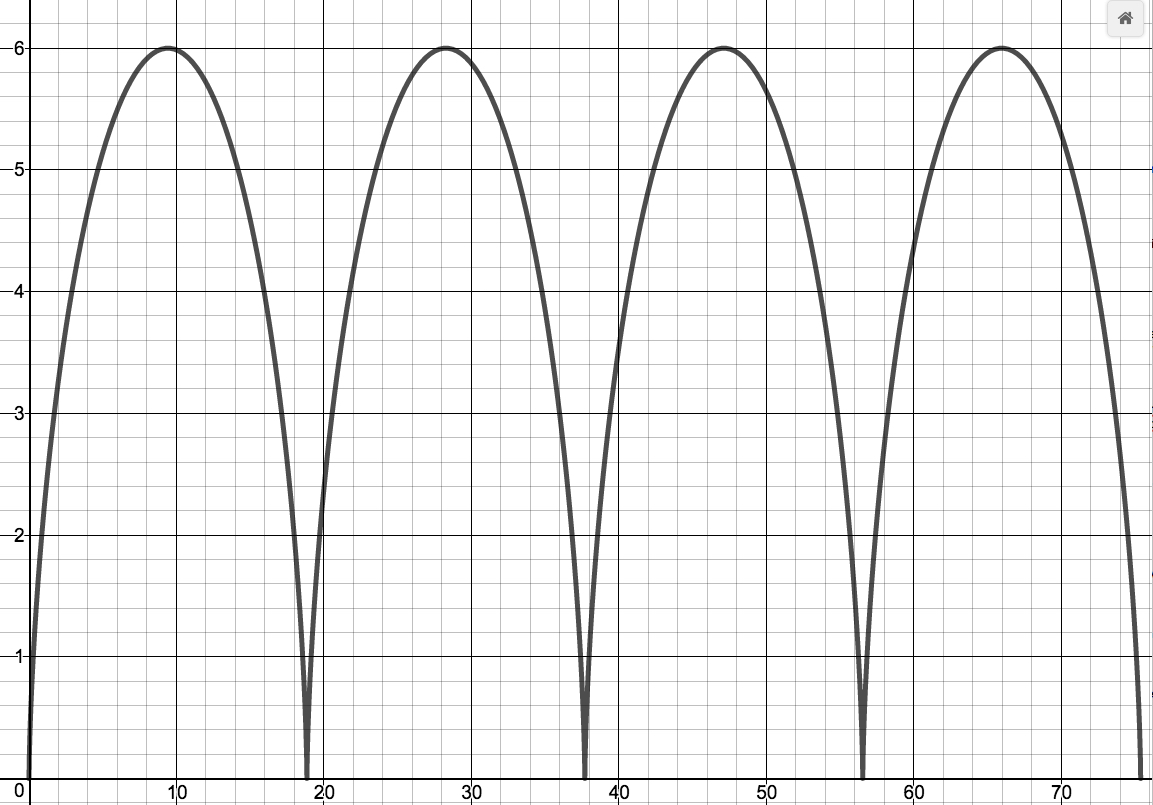
\includegraphics[width=4in]{./ParametricEquationsGraphics/cycloid.jpg}

\end{center}

We see the equations create a series of `arches' and can (partially) verify the reasonableness the graph by finding the $x$-intercepts.  To do this, we set $y = 3(1-\cos(t)) = 0$, which amounts to solving $\cos(t) = 1$.  

\smallskip

We get $t = 2 \pi k$ and since $t \geq 0$, $k$ can be any \textit{nonnegative} integer.  Substituting a few of these values for $t$, $t = 0$, $t = 2\pi$, $t = 4\pi$, and $t=6\pi$ into the equations $x = 3(t -\sin(t))$ and $y = 3(1-\cos(t))$ we obtain the points $(0,0)$, $(6\pi, 0) \approx (18.85, 0)$,  $(12 \pi,0) \approx (37.70, 0)$ and $(18\pi, 0) \approx ( 56.55 , 0)$, which match the graph. In general, the $x$-intercepts are $(6\pi k, 0)$ for nonnegative integers $k$.  We leave the details to the reader.

\smallskip

We note it is also possible to analytically determine  the (local) maximums of the graph using the techniques demonstrated in Example \ref{parametrictorect}  by analyzing $y = 3(1-\cos(t))$ .   The maximums occur when $t = (2k +1) \pi k$ where $k$ is a nonnegative integer, which isn't too surprising just looking at the problem from a  symmetry perspective.  Substituting these values for $t$ into our equations for $x$ and $y$ produce points of the form $(3(2k+1) \pi, 6)$.  We leave the details to the reader.  \qed

\end{example}



\newpage

\subsection{Exercises}


%% SKIPPED %% In Exercises \ref{paraplotfirst} - \ref{paraplotlast}, plot the set of parametric equations by hand. Be sure to indicate the orientation imparted on the curve by the parametrization.  

\begin{multicols}{2} \raggedcolumns 

\begin{enumerate}

\item ${\displaystyle \left\{ \begin{array}{l} x = 4t-3 \\ y = 6t-2 \end{array} \right. \vspace{.25in} \mbox{for } 0 \leq t \leq 1}$ \label{paraplotfirst}
\item ${\displaystyle \left\{ \begin{array}{l} x = 4t-1 \\ y = 3-4t \end{array} \right. \vspace{.25in} \mbox{for } 0 \leq t \leq 1}$

\setcounter{HW}{\value{enumi}}
\end{enumerate}
\end{multicols}

\begin{multicols}{2} \raggedcolumns 
\begin{enumerate}
\setcounter{enumi}{\value{HW}}
\item ${\displaystyle \left\{ \begin{array}{l} x = 2t \\ y = t^2 \end{array} \right. \vspace{.25in} \mbox{for } -1 \leq t \leq 2}$
\item ${\displaystyle \left\{ \begin{array}{l} x = t-1 \\ y = 3+2t-t^2 \end{array} \right. \vspace{.25in} \mbox{for } 0 \leq t \leq 3}$

\setcounter{HW}{\value{enumi}}
\end{enumerate}
\end{multicols}



\begin{multicols}{2} \raggedcolumns 
\begin{enumerate}
\setcounter{enumi}{\value{HW}}
\item ${\displaystyle \left\{ \begin{array}{l} x = t^2+2t+1 \\[3pt] y = t+1 \end{array} \right. \vspace{.25in} \mbox{for } t \leq 1}$
\item ${\displaystyle \left\{ \begin{array}{l} x = \frac{1}{9}\left(18-t^2\right) \\[3pt] y = \frac{1}{3} t \end{array} \right. \vspace{.25in} \mbox{for } t \geq -3}$

\setcounter{HW}{\value{enumi}}
\end{enumerate}
\end{multicols}


\begin{multicols}{2} \raggedcolumns 
\begin{enumerate}
\setcounter{enumi}{\value{HW}}

\item ${\displaystyle \left\{ \begin{array}{l} x = t \\ y = t^3 \end{array} \right. \vspace{.25in} \mbox{for } -\infty < t < \infty}$
\item ${\displaystyle \left\{ \begin{array}{l} x = t^3 \\ y = t \end{array} \right. \vspace{.25in} \mbox{for } -\infty < t < \infty}$

\setcounter{HW}{\value{enumi}}
\end{enumerate}
\end{multicols}

\begin{multicols}{2} \raggedcolumns 
\begin{enumerate}
\setcounter{enumi}{\value{HW}}
\item ${\displaystyle \left\{ \begin{array}{l} x = \cos(t) \\ y = \sin(t) \end{array} \right. \vspace{.25in} \mbox{for } -\dfrac{\pi}{2} \leq t \leq \dfrac{\pi}{2}}$
\item ${\displaystyle \left\{ \begin{array}{l} x = 3\cos(t) \\ y = 3\sin(t) \end{array} \right. \vspace{.25in} \mbox{for } 0 \leq t \leq \pi}$


\setcounter{HW}{\value{enumi}}
\end{enumerate}
\end{multicols}



\begin{multicols}{2} \raggedcolumns 
\begin{enumerate}
\setcounter{enumi}{\value{HW}}

\item ${\displaystyle \left\{ \begin{array}{l} x = -1+ 3\cos(t) \\ y = 4\sin(t) \end{array} \right. \vspace{.25in} \mbox{for } 0 \leq t \leq 2\pi}$
\item ${\displaystyle \left\{ \begin{array}{l} x = 3\cos(t) \\ y = 2\sin(t)+1 \end{array} \right. \vspace{.25in} \mbox{for } \dfrac{\pi}{2} \leq t \leq 2\pi}$

\setcounter{HW}{\value{enumi}}
\end{enumerate}
\end{multicols}

\begin{multicols}{2} \raggedcolumns 
\begin{enumerate}
\setcounter{enumi}{\value{HW}}

\item ${\displaystyle \left\{ \begin{array}{l} x = 2\cos(t) \\ y = \sec(t) \end{array} \right. \vspace{.25in} \mbox{for } 0 \leq t < \dfrac{\pi}{2}}$
\item ${\displaystyle \left\{ \begin{array}{l} x = 2\tan(t) \\ y = \cot(t) \end{array} \right. \vspace{.25in} \mbox{for } 0 < t < \dfrac{\pi}{2}}$

\setcounter{HW}{\value{enumi}}
\end{enumerate}
\end{multicols}


\begin{multicols}{2} \raggedcolumns 
\begin{enumerate}
\setcounter{enumi}{\value{HW}}

\item ${\displaystyle \left\{ \begin{array}{l} x = \sec(t) \\ y = \tan(t) \end{array} \right. \vspace{.25in} \mbox{for } -\dfrac{\pi}{2} < t < \dfrac{\pi}{2}}$
\item ${\displaystyle \left\{ \begin{array}{l} x = \sec(t) \\ y = \tan(t) \end{array} \right. \vspace{.25in} \mbox{for } \dfrac{\pi}{2} < t < \dfrac{3\pi}{2}}$

\setcounter{HW}{\value{enumi}}
\end{enumerate}
\end{multicols}

\begin{multicols}{2} \raggedcolumns 
\begin{enumerate}
\setcounter{enumi}{\value{HW}}

\item ${\displaystyle \left\{ \begin{array}{l} x = \tan(t) \\ y = 2\sec(t) \end{array} \right. \vspace{.25in} \mbox{for } -\dfrac{\pi}{2} < t < \dfrac{\pi}{2}}$
\item ${\displaystyle \left\{ \begin{array}{l} x = \tan(t) \\ y = 2\sec(t) \end{array} \right. \vspace{.25in} \mbox{for } \dfrac{\pi}{2} < t < \dfrac{3\pi}{2}}$

\setcounter{HW}{\value{enumi}}
\end{enumerate}
\end{multicols}


\begin{multicols}{2} \raggedcolumns 
\begin{enumerate}
\setcounter{enumi}{\value{HW}}

\item ${\displaystyle \left\{ \begin{array}{l} x = \cos(t) \\ y = t \end{array} \right. \vspace{.25in} \mbox{for } 0 \leq t \leq \pi}$
\item ${\displaystyle \left\{ \begin{array}{l} x = \sin(t) \\ y = t \end{array} \right. \vspace{.25in} \mbox{for } -\dfrac{\pi}{2} \leq t \leq \dfrac{\pi}{2}}$ \label{paraplotlast}

\setcounter{HW}{\value{enumi}}
\end{enumerate}
\end{multicols}

\newpage

In the same way (and for the same reason) we took the time on page \pageref{polargraphscalculator} in Section \ref{PolarGraphs} to show how to graph polar equations using a graphing calculator, we take a few moments here to explain how to graph a system of parametric equations using a calculator.  Our task is to graph the cycloid from Example \ref{cycloidex},  $\left\{ x = 3(t -\sin(t)), \, y = 3(1-\cos(t)) \right.$ for $t \geq 0$ using a graphing calculator.

\smallskip

We first must ensure that the calculator is in `Parametric Mode' and `radian mode' when we enter the equations and advance to the `Window' screen. 

\begin{center}

\begin{tabular}{cc}

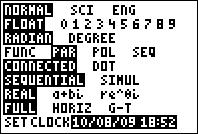
\includegraphics[width=2in]{./ParametricEquationsGraphics/Parametric01.jpg} &
\hspace{0.75in} 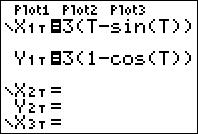
\includegraphics[width=2in]{./ParametricEquationsGraphics/Parametric02.jpg} \\

\end{tabular} 

\end{center}

Our next step is to find appropriate bounds on the parameter, $t$, as well as for $x$ and $y$.   We know that one full revolution of the circle occurs over the interval $0 \leq t < 2\pi$, so it seems reasonable to keep these as our bounds on $t$.  The `Tstep' seems reasonably small -- too large a value here can lead to incorrect graphs.\footnote{Again, see page \pageref{polargraphscalculator} in Section \ref{PolarGraphs}.}  We know from our derivation of the equations of the cycloid that the center of the generating circle has coordinates $(r\theta,r)  = (3t,3)$.  Since  $t$ ranges between $0$ and $2\pi$, we set $x$ to range between $0$ and $6\pi$.  The values of $y$ go from the bottom of the circle to the top, so $y$ ranges between $0$ and $6$.

\begin{center}
\begin{tabular}{cc}

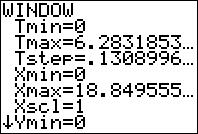
\includegraphics[width=2in]{./ParametricEquationsGraphics/Parametric03.jpg} &
\hspace{0.75in} 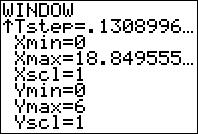
\includegraphics[width=2in]{./ParametricEquationsGraphics/Parametric04.jpg} \\

\end{tabular} 


\end{center}

Below we graph the cycloid with these settings, and then extend $t$ to range from $0$ to $6\pi$ which forces $x$ to range from $0$ to $18\pi$ yielding three arches of the cycloid.\footnote{It is instructive to note that keeping the $y$ settings between 0 and 6 skews the aspect ratio of the cycloid.  Using the `Zoom Square' feature on the graphing calculator gives a true geometric perspective of the three arches.}

\begin{center}

\begin{tabular}{cc}

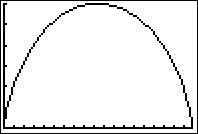
\includegraphics[width=2in]{./ParametricEquationsGraphics/Parametric05.jpg} &
\hspace{0.75in} 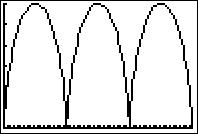
\includegraphics[width=2in]{./ParametricEquationsGraphics/Parametric06.jpg} \\


\end{tabular} 
\end{center}


In Exercises \ref{paracalcfirst} - \ref{paracalclast}, plot the set of parametric equations with the help of a graphing utility.  Be sure to indicate the orientation imparted on the curve by the parametrization.  

\begin{multicols}{2} \raggedcolumns 
\begin{enumerate}
\setcounter{enumi}{\value{HW}}


\item ${\displaystyle \left\{ \begin{array}{l} x = t^{3} - 3t \\ y = t^{2} - 4 \end{array} \right. \vspace{.25in} \mbox{for } -2 \leq t \leq 2}$ \label{paracalcfirst}
\item ${\displaystyle \left\{ \begin{array}{l} x = 4\cos^{3}(t) \\ y = 4\sin^{3}(t) \end{array} \right. \vspace{.25in} \mbox{for } 0 \leq t \leq 2\pi}$

\setcounter{HW}{\value{enumi}}
\end{enumerate}
\end{multicols}

\begin{multicols}{2} \raggedcolumns 
\begin{enumerate}
\setcounter{enumi}{\value{HW}}


\item ${\displaystyle \left\{ \begin{array}{l} x = e^{t} + e^{-t} \\ y = e^{t} - e^{-t} \end{array} \right. \vspace{.25in} \mbox{for }  -2 \leq t \leq 2}$
\item ${\displaystyle \left\{ \begin{array}{l} x = \cos(3t) \\ y = \sin(4t) \end{array} \right. \vspace{.25in} \mbox{for } 0 \leq t \leq 2\pi}$ \label{paracalclast}

\setcounter{HW}{\value{enumi}}
\end{enumerate}
\end{multicols}


In Exercises \ref{findparamfirst} - \ref{findparamlast}, find a parametric description for the given oriented curve.

\begin{enumerate}

\setcounter{enumi}{\value{HW}}

\item  the directed line segment from $(3,-5)$ to $(-2,2)$ \label{findparamfirst}

\item  the directed line segment from $(-2,-1)$ to $(3, -4)$ 

\item  the curve $y = 4-x^2$ from $(-2,0)$ to $(2,0)$.

\item   the curve $y = 4-x^2$ from $(-2,0)$ to $(2,0)$ \\
(Shift the parameter so  $t=0$ corresponds to $(-2,0)$.)

\item  the curve $x = y^2 - 9$ from $(-5,-2)$ to $(0,3)$.

\item  the curve $x = y^2 - 9$ from $(0,3)$ to $(-5,-2)$.\\
(Shift the parameter so  $t=0$ corresponds to $(0,3)$.)

\item   the circle $x^2 + y^2 = 25$, oriented counter-clockwise

\item   the circle $(x-1)^2 + y^2 = 4$, oriented counter-clockwise

\item   the circle $x^2 + y^2 - 6y = 0$, oriented counter-clockwise

\item   the circle $x^2 + y^2 - 6y = 0$, oriented \emph{clockwise}\\
(Shift the parameter so  $t$ begins at $0$.)

\item   the circle $(x-3)^2 + (y+1)^2 = 117$, oriented counter-clockwise

\item   the ellipse $(x-1)^2 + 9y^2 = 9$, oriented counter-clockwise

\item   the ellipse $9x^2 + 4y^2 + 24y =0$, oriented counter-clockwise

\item   the ellipse $9x^2 + 4y^2 + 24y =0$, oriented clockwise  \\
(Shift the parameter so $t=0$ corresponds to  $(0,0)$.)

\item  the triangle with vertices $(0,0)$, $(3,0)$, $(0,4)$, oriented counter-clockwise \\
(Shift the parameter so $t=0$ corresponds to $(0,0)$.) \label{findparamlast}

\setcounter{HW}{\value{enumi}}

\end{enumerate}

\begin{enumerate}

\setcounter{enumi}{\value{HW}}

\item Use parametric equations and a graphing utility to graph the inverse of $f(x) = x^{3} + 3x - 4$.

\item  Every polar curve $r = f(\theta)$ can be translated to a system of parametric equations with parameter $\theta$ by $\left\{ x = r\cos(\theta) = f(\theta) \cos(\theta), \, y = r \sin(\theta) = f(\theta) \sin(\theta) \right.$.  Convert $r = 6\cos(2\theta)$ to a system of parametric equations. Check your answer by graphing $r = 6\cos(2\theta)$ by hand using the techniques presented in Section \ref{PolarGraphs} and then graphing the parametric equations you found using a graphing utility.


\item  Use your results from Exercises \ref{heightlondoneye} and \ref{leftrightlondoneye} in Section \ref{Sinusoid} to find the parametric equations which model a passenger's position as they ride the \href{http://en.wikipedia.org/wiki/London_Eye}{\underline{London Eye}}. 




\setcounter{HW}{\value{enumi}}
\end{enumerate}

\phantomsection
\label{projectoilemotion}

Suppose an object, called a projectile, is launched into the air.  Ignoring everything except the force gravity, the path of the projectile is given by\footnote{A nice mix of vectors and Calculus are needed to derive this.}

\[ \left\{ \begin{array}{l} x =   v_{\text{\tiny $0$}} \cos(\theta) \, t \\ [3pt]
															y = -\dfrac{1}{2} g t^2 +  v_{\text{\tiny $0$}} \sin(\theta) \, t + s_{\text{\tiny $0$}} \\ \end{array} \right. \; \text{for} \; 0 \leq t \leq T \]

where  $v_{\text{\tiny $0$}}$ is the initial speed of the object, $\theta$ is the angle from the horizontal at which the projectile is launched,\footnote{We've seen this before.  It's the angle of elevation which was defined on page \pageref{angleofelevation}.} $g$ is the acceleration due to gravity,  $s_{\text{\tiny $0$}}$ is the initial height of the projectile above the ground and $T$ is the time when the object returns to the ground.  (See the figure below.)

\begin{center}

\begin{mfpic}[20]{-1}{9}{-1}{7}
\axes
\tlabel[cc](9,-0.5){\scriptsize $x$}
\tlabel[cc](0.5,7){\scriptsize $y$}
\dashed \polyline{(0,4), (1.5,4)}
\tlabelsep{5pt}
\axislabels{y}{{\scriptsize $s_{\text{\tiny $0$}}$} 4}
\point[4pt]{(0,4), (5.98,0)}
\arrow \shiftpath{(0,4)}  \parafcn{5, 55, 5}{0.75*dir(t)}
\tlabel[cc](1,4.5){\scriptsize $\theta$}
\tlabel[cc](5.98,-0.5){\scriptsize $(x(T), 0)$}
\penwd{1.25pt}
\arrow \parafcn{0,0.75,0.1}{(3.5*t, 6.062*t+4-(4.9*(t**2)))}
\parafcn{0.75,1.71,0.1}{(3.5*t, 6.062*t+4-(4.9*(t**2)))}

\end{mfpic}


\end{center}

\begin{enumerate}
\setcounter{enumi}{\value{HW}}

\item  Carl's friend Jason competes in Highland Games Competitions across the country.  In one event, the `hammer throw',  he throws a 56 pound weight for distance. If the weight is released $6$ feet above the ground at an angle of $42^{\circ}$ with respect to the horizontal with an initial speed of $33$ feet per second, find the parametric equations for the flight of the hammer.  (Here, use $g = 32 \frac{\text{ft.}}{s^2}$.) When will the hammer hit the ground?  How far away will it hit the ground? Check your answer using a graphing utility.

\item  \label{projectileeliminate} Eliminate the parameter in the equations for projectile motion to show that the path of the projectile follows the curve \[y = -\dfrac{g \sec^{2}(\theta)}{2 v_{\text{\tiny$0$}}^2} x^2 + \tan(\theta) x + s_{\text{\tiny $0$}}\] Use the vertex formula (Equation \ref{vertexofquadraticfunctions}) to show the maximum height of the projectile is \[y = \dfrac{v_{\text{\tiny$0$}}^2 \sin^{2}(\theta)}{2g} + s_{\text{\tiny $0$}} \quad \text{when} \quad x = \dfrac{v_{\text{\tiny$0$}}^2 \sin(2\theta) }{2g}\] 

\item  In another event, the `sheaf toss', Jason throws a  20 pound weight for height.  If the weight is released  5 feet above the ground at an angle of $85^{\circ}$ with respect to the horizontal and the sheaf reaches a maximum height of 31.5 feet, use your results from part  \ref{projectileeliminate} to determine how fast the sheaf was launched into the air.  (Once again, use $g = 32 \frac{\text{ft.}}{s^2}$.)

\item  Suppose $\theta = \frac{\pi}{2}$. (The projectile was launched vertically.) Simplify the general parametric formula given for $y(t)$ above using  $g = 9.8 \, \frac{m}{s^2}$ and compare that to the formula for $s(t)$ given in Exercise \ref{whatgoesup} in Section \ref{QuadraticFunctions}.  What is $x(t)$ in this case?

\item  If $f$ and $g$ are functions, explain why the function $\vec{r}(t) = \left<f(t), g(t) \right>$ is a function. The function $\vec{r}$ is called a \index{function ! vector-valued}\index{vector-valued function}\textbf{vector-valued function} since it matches real number inputs, $t$, with vector outputs, $\vec{r}(t)$.   Explain why when the vectors  $\vec{r}(t)$ are plotted in standard position, their terminal points trace out the curve described parametrically by the system of equations:  $\left\{ x = f(t) \, y =  g(t) \right.$  (In Calculus, you will see  systems of parametric equations `packaged' together using vectors.)

\setcounter{HW}{\value{enumi}}
\end{enumerate}


\phantomsection
\label{hyperboliccosinesine} 

In Exercises \ref{hyperbolicfirst} - \ref{hyperboliclast}, we explore the  \textbf{hyperbolic cosine}\index{hyperbolic cosine} function, denoted $\cosh(t)$, and the \textbf{hyperbolic sine}\index{hyperbolic sine}
function, denoted $\sinh(t)$, defined below:

\[ \begin{array}{ccc}

\cosh(t) = \dfrac{e^{t} + e^{-t}}{2} & 
\text{and} & \sinh(t) = \dfrac{e^{t} - e^{-t}}{2} \\

\end{array} \]

\begin{enumerate}
\setcounter{enumi}{\value{HW}}

\item  Using a graphing utility as needed, verify the following:  \label{hyperbolicfirst}

\begin{enumerate}

\item the domain of $\cosh(t)$ is $(-\infty, \infty)$ and the range of $\cosh(t)$ is $[1,\infty)$.

\item  the domain and range  of $\sinh(t)$ are both $(-\infty, \infty)$.

\end{enumerate}

\item  Show that $\left\{ x(t) = \cosh(t), \, y(t) = \sinh(t) \right.$ parametrize the right half of the `unit' hyperbola $x^2 - y^2 = 1$.  (Hence the use of the adjective `hyperbolic.')

\item  Compare and contrast the definitions of $\cosh(t)$ and $\sinh(t)$ to the formulas for $\cos(t)$ and $\sin(t)$ given in Exercise \ref{expformcosandsin} in Section \ref{PolarComplex}.

\item \label{andtheresthyperbolic} Four other hyperbolic functions are waiting to be defined:  the hyperbolic secant $\text{sech}(t)$, the hyperbolic cosecant $\text{csch}(t)$, the hyperbolic tangent $\tanh(t)$ and the hyperbolic cotangent $\coth(t)$.  Define these functions in terms of $\cosh(t)$ and $\sinh(t)$, then convert them to formulas involving $e^{t}$ and $e^{-t}$.  Consult a suitable reference (a Calculus book, or this entry on the \href{http://en.wikipedia.org/wiki/Hyperbolic_function}{\underline{hyperbolic functions}}) and spend some time reliving the thrills of trigonometry with these `hyperbolic' functions.

\item  If these functions look familiar, they should.  Enjoy some nostalgia and revisit Exercise \ref{catenary} in Section \ref{ExpLogApplications}, Exercise \ref{hyperbolicsine} in Section \ref{ExponentialEquationsandInequalities} and the  answer to Exercise \ref{inversehyptangent} in Section \ref{LogarithmicEquationsandInequalities}. \label{hyperboliclast}

\end{enumerate}

\newpage

\subsection{Answers}

\begin{multicols}{2} \raggedcolumns 
\begin{enumerate}

\item ${\displaystyle \left\{ \begin{array}{l} x = 4t-3 \\ y = 6t-2 \end{array} \right. \vspace{.25in} \mbox{for } 0 \leq t \leq 1}$

\begin{mfpic}[15]{-4}{2}{-3}{5}
\axes
\tlabel[cc](2,-0.5){\scriptsize $x$}
\tlabel[cc](0.5,5){\scriptsize $y$}
\xmarks{-3,-2,-1,1}
\ymarks{-2,-1,1,2,3,4}
\point[4pt]{(-3,-2), (1,4)}
\tlpointsep{4pt}
\scriptsize
\axislabels {x}{{$-3 \hspace{6pt}$} -3,{$-2 \hspace{6pt}$} -2,{$-1 \hspace{6pt}$} -1, {$1$} 1}
\axislabels {y}{{$-1$} -1,{$-2$} -2, {$1$} 1,{$2$} 2,{$3$} 3,{$4$} 4}
\normalsize
\penwd{1.25pt}
\arrow \parafcn{0,0.5,0.1}{(4*t-3,6*t-2)}
\parafcn{0.5,1,0.1}{(4*t-3,6*t-2)}
\end{mfpic}


\item ${\displaystyle \left\{ \begin{array}{l} x = 4t-1 \\ y = 3-4t \end{array} \right. \vspace{.25in} \mbox{for } 0 \leq t \leq 1}$


\begin{mfpic}[15]{-2}{4}{-2}{4}
\axes
\tlabel[cc](4,-0.5){\scriptsize $x$}
\tlabel[cc](0.5,4){\scriptsize $y$}
\xmarks{-1,1,2,3}
\ymarks{-1,1,2,3}
\point[4pt]{(-1,3), (3,-1)}
\tlpointsep{4pt}
\scriptsize
\axislabels {x}{{$-1 \hspace{6pt}$} -1, {$1$} 1, {$2$} 2,{$3$} 3}
\axislabels {y}{{$-1$} -1, {$1$} 1,{$2$} 2,{$3$} 3}
\normalsize
\penwd{1.25pt}
\arrow \parafcn{0,0.5,0.1}{(4*t-1,3-4*t)}
\parafcn{0.5,1,0.1}{(4*t-1,3-4*t)}
\end{mfpic}
\setcounter{HW}{\value{enumi}}
\end{enumerate}
\end{multicols}



\begin{multicols}{2} \raggedcolumns 
\begin{enumerate}
\setcounter{enumi}{\value{HW}}

\item ${\displaystyle \left\{ \begin{array}{l} x = 2t \\ y = t^2 \end{array} \right. \vspace{.25in} \mbox{for } -1 \leq t \leq 2}$

\begin{mfpic}[15]{-3}{5}{-1}{5}
\axes
\tlabel[cc](5,-0.5){\scriptsize $x$}
\tlabel[cc](0.5,5){\scriptsize $y$}
\xmarks{-2,-1,1,2,3,4}
\ymarks{1,2,3,4}
\point[4pt]{(-2,1), (0,0), (4,4)}
\tlpointsep{4pt}
\scriptsize
\axislabels {x}{{$-3 \hspace{6pt}$} -3,{$-2 \hspace{6pt}$} -2,{$-1 \hspace{6pt}$} -1, {$1$} 1, {$2$} 2,{$3$} 3,{$4$} 4}
\axislabels {y}{{$1$} 1,{$2$} 2,{$3$} 3,{$4$} 4}
\normalsize
\penwd{1.25pt}
\arrow \parafcn{-1,-0.5,0.1}{(2*t,(t**2))}
\arrow \parafcn{-0.5,1,0.1}{(2*t,(t**2))}
\parafcn{1,2,0.1}{(2t,t**2)}
\end{mfpic}


\item ${\displaystyle \left\{ \begin{array}{l} x = t-1 \\ y = 3+2t-t^2 \end{array} \right. \vspace{.25in} \mbox{for } 0 \leq t \leq 3}$


\begin{mfpic}[15]{-2}{3}{-1}{5}
\axes
\tlabel[cc](4,-0.5){\scriptsize $x$}
\tlabel[cc](0.5,5){\scriptsize $y$}
\xmarks{-1,1,2}
\ymarks{1,2,3,4}
\point[4pt]{(-1,3), (0,4), (2,0)}
\tlpointsep{4pt}
\scriptsize
\axislabels {x}{{$-1 \hspace{6pt}$} -1, {$1$} 1, {$2$} 2}
\axislabels {y}{{$1$} 1,{$2$} 2,{$3$} 3,{$4$} 4}
\normalsize
\penwd{1.25pt}
\arrow \parafcn{0,0.5,0.1}{(t-1,3+2*t-(t**2))}
\arrow \parafcn{0.5,2,0.1}{(t-1,3+2*t-(t**2))}
\parafcn{2,3,0.1}{(t-1,3+2*t-(t**2))}

\end{mfpic}

\setcounter{HW}{\value{enumi}}
\end{enumerate}
\end{multicols}


\begin{multicols}{2} \raggedcolumns 
\begin{enumerate}
\setcounter{enumi}{\value{HW}}

\item ${\displaystyle \left\{ \begin{array}{l} x = t^2+2t+1 \\ y = t+1 \end{array} \right. \vspace{.25in} \mbox{for } t \leq 1}$

\begin{mfpic}[15]{-1}{6}{-3}{3}
\axes
\tlabel[cc](6,-0.5){\scriptsize $x$}
\tlabel[cc](0.5,3){\scriptsize $y$}
\xmarks{1,2,3,4,5}
\ymarks{-2,-1,1,2}
\point[4pt]{(4,2), (0,0), (4,-2)}
\tlpointsep{4pt}
\scriptsize
\axislabels {x}{ {$1$} 1, {$2$} 2,{$3$} 3,{$4$} 4,{$5$} 5}
\axislabels {y}{{$-2$} -2,{$-1$} -1,{$1$} 1,{$2$} 2,{$3$}}
\normalsize
\penwd{1.25pt}
\parafcn{0,1,0.1}{((t**2)+(2*t)+1,t+1)}
\arrow \parafcn{-2,0,0.1}{((t**2)+(2*t)+1,t+1)}
\arrow \parafcn{-3.25,-2,0.1}{((t**2)+(2*t)+1,t+1)}
\arrow \parafcn{-3.44,-3.25,0.1}{((t**2)+(2*t)+1,t+1)}
\end{mfpic} 

\item ${\displaystyle \left\{ \begin{array}{l} x = \frac{1}{9}\left(18-t^2\right) \\ y = \frac{1}{3} t \end{array} \right. \vspace{.25in} \mbox{for } t \geq -3}$



\begin{mfpic}[15]{-4}{3}{-2}{3}
\axes
\tlabel[cc](3,-0.5){\scriptsize $x$}
\tlabel[cc](0.5,3){\scriptsize $y$}
\xmarks{-3,-2,-1,1,2}
\ymarks{-1,1,2}
\point[4pt]{(1,-1), (2,0), (-2,2)}
\tlpointsep{4pt}
\scriptsize
\axislabels {x}{{$-3 \hspace{6pt}$} -3,{$-2 \hspace{6pt}$} -2,{$-1 \hspace{6pt}$} -1, {$1$} 1, {$2$} 2}
\axislabels {y}{{$-1$} -1,{$1$} 1,{$2$} 2}
\normalsize
\penwd{1.25pt}
\arrow \parafcn{-3,-1.5,0.1}{((18-(t**2))/9,t/3)}
\arrow \parafcn{-1.5,3,0.1}{((18-(t**2))/9,t/3)}
\arrow \parafcn{3,6.5,0.1}{((18-(t**2))/9,t/3)}

\end{mfpic}

\setcounter{HW}{\value{enumi}}
\end{enumerate}
\end{multicols}


\pagebreak


\begin{multicols}{2} \raggedcolumns 
\begin{enumerate}
\setcounter{enumi}{\value{HW}}

\item ${\displaystyle \left\{ \begin{array}{l} x = t \\ y = t^3 \end{array} \right. \vspace{.25in} \mbox{for } -\infty < t < \infty}$


\begin{mfpic}[15]{-2}{2}{-5}{5}
\axes
\tlabel[cc](2,-0.5){\scriptsize $x$}
\tlabel[cc](0.5,5){\scriptsize $y$}
\xmarks{-1,1}
\ymarks{-4,-3,-2,-1,1,2,3,4}
\point[4pt]{(-1,-1), (0,0), (1,1)}
\tlpointsep{4pt}
\scriptsize
\axislabels {x}{{$-1 \hspace{6pt}$} -1, {$1$} 1}
\axislabels {y}{{$-4$} -4,{$-3$} -3,{$-2$} -2,{$-1$} -1,{$1$} 1,{$2$} 2,{$3$} 3,{$4$} 4}
\normalsize
\penwd{1.25pt}
\arrow \parafcn{-1.7,-1.25,0.1}{(t, t**3)}
\arrow \parafcn{-1.25,1.25,0.1}{(t, t**3)}
\arrow \parafcn{1.25,1.7,0.1}{(t, t**3)}
\end{mfpic}


\item ${\displaystyle \left\{ \begin{array}{l} x = t^3 \\ y = t \end{array} \right. \vspace{.25in} \mbox{for } -\infty < t < \infty}$

\begin{mfpic}[15]{-5}{5}{-2}{2}
\axes
\tlabel[cc](5,-0.5){\scriptsize $x$}
\tlabel[cc](0.5,2){\scriptsize $y$}
\xmarks{-4,-3,-2,-1,1,2,3,4}
\ymarks{-1,1}
\point[4pt]{(-1,-1), (0,0), (1,1)}
\tlpointsep{4pt}
\scriptsize
\axislabels {y}{{$-1$} -1, {$1$} 1}
\axislabels {x}{{$-4 \hspace{6pt}$} -4,{$-3 \hspace{6pt}$} -3,{$-2 \hspace{6pt}$} -2,{$-1 \hspace{6pt}$} -1,{$1$} 1,{$2$} 2,{$3$} 3,{$4$} 4}
\normalsize
\penwd{1.25pt}
\arrow \parafcn{-1.7,-1.25,0.1}{(t**3, t)}
\arrow \parafcn{-1.25,1.25,0.1}{(t**3, t)}
\arrow \parafcn{1.25,1.7,0.1}{(t**3, t)}
\end{mfpic}


\setcounter{HW}{\value{enumi}}
\end{enumerate}
\end{multicols}



\begin{multicols}{2}

\begin{enumerate}

\setcounter{enumi}{\value{HW}}
\item ${\displaystyle \left\{ \begin{array}{l} x = \cos(t) \\ y = \sin(t) \end{array} \right. \vspace{.25in} \mbox{for } -\dfrac{\pi}{2} \leq t \leq \dfrac{\pi}{2}}$

\begin{mfpic}[10]{-5}{5}{-5}{5}
\axes
\tlabel[cc](5,-0.5){\scriptsize $x$}
\tlabel[cc](0.5,5){\scriptsize $y$}
\point[4pt]{(0,-4), (4,0), (0,4)}
\xmarks{-4,4}
\ymarks{-4,4}
\tlpointsep{4pt}
\scriptsize
\axislabels {x}{{$-1 \hspace{6pt}$} -4, {$1$} 4}
\axislabels {y}{{$-1$} -4, {$1$} 4}
\normalsize
\penwd{1.25pt}
\arrow \parafcn{-1.57,-0.78,0.1}{(4*cos(t),4*sin(t))}
\arrow \parafcn{-0.78,0.78,0.1}{(4*cos(t),4*sin(t))}
\parafcn{0.78,1.57,0.1}{(4*cos(t),4*sin(t))}
\end{mfpic} 


\item ${\displaystyle \left\{ \begin{array}{l} x = 3\cos(t) \\ y = 3\sin(t) \end{array} \right. \vspace{.25in} \mbox{for } 0 \leq t \leq \pi}$

\begin{mfpic}[15]{-4}{4}{-1}{4}
\axes
\tlabel[cc](4,-0.5){\scriptsize $x$}
\tlabel[cc](0.5,4){\scriptsize $y$}
\point[4pt]{(-3,0), (3,0), (0,3)}
\xmarks{-3,-2,-1,1,2,3}
\ymarks{1,2,3}
\tlpointsep{4pt}
\scriptsize
\axislabels {x}{{$-3 \hspace{6pt}$} -3, {$-2 \hspace{6pt}$} -2,{$-1 \hspace{6pt}$} -1,{$1$} 1,{$2$} 2,{$3$} 3}
\axislabels {y}{{$1$} 1,{$2$} 2,{$3$} 3}
\normalsize
\penwd{1.25pt}
\arrow \parafcn{0,0.78,0.1}{(3*cos(t),3*sin(t))}
\arrow \parafcn{0.78,2.36,0.1}{(3*cos(t),3*sin(t))}
\parafcn{2.36,3.14,0.1}{(3*cos(t),3*sin(t))}
\end{mfpic} 

\setcounter{HW}{\value{enumi}}
\end{enumerate}
\end{multicols}




\begin{multicols}{2}
\begin{enumerate}
\setcounter{enumi}{\value{HW}}

\item  ${\displaystyle \left\{ \begin{array}{l} x = -1+3\cos(t) \\ y = 4\sin(t) \end{array} \right. \vspace{.25in} \mbox{for } 0 \leq t \leq 2\pi}$

\begin{mfpic}[15]{-5}{3}{-5}{5}
\axes
\tlabel[cc](3,-0.5){\scriptsize $x$}
\tlabel[cc](0.5,5){\scriptsize $y$}
\point[4pt]{(2,0), (-1,4), (-4,0), (-1,-4)}
\xmarks{-4,-3,-2,-1,1,2}
\ymarks{-4,-3,-2,-1,1,2,3,4}
\tlpointsep{4pt}
\scriptsize
\axislabels {x}{{$-4 \hspace{6pt}$} -4,{$-3 \hspace{6pt}$} -3,{$-2 \hspace{6pt}$} -2, {$-1 \hspace{6pt}$} -1,{$1$} 1,{$2$} 2}
\axislabels {y}{{$-4$} -4, {$-3$} -3,{$-2$} -2,{$-1$} -1,{$1$} 1,{$2$} 2,{$3$} 3,{$4$} 4}
\normalsize
\penwd{1.25pt}
\arrow \parafcn{0,0.78,0.1}{(3*cos(t)-1,4*sin(t))}
\arrow \parafcn{0.78,2.36, 0.1}{(3*cos(t)-1,4*sin(t))}
\arrow \parafcn{2.36,3.93, 0.1}{(3*cos(t)-1,4*sin(t))}
\arrow \parafcn{3.93,5.5, 0.1}{(3*cos(t)-1,4*sin(t))}
\parafcn{5.5,6.28, 0.1}{(3*cos(t)-1,4*sin(t))}
\end{mfpic} 

\item ${\displaystyle \left\{ \begin{array}{l} x = 3\cos(t) \\ y = 2\sin(t)+1 \end{array} \right. \vspace{.25in} \mbox{for } \dfrac{\pi}{2} \leq t \leq 2\pi}$

\begin{mfpic}[15]{-4}{4}{-2}{4}
\axes
\tlabel[cc](4,-0.5){\scriptsize $x$}
\tlabel[cc](0.5,4){\scriptsize $y$}
\point[4pt]{(0,3), (-3,1), (0,-1), (3,1)}
\xmarks{-3,-2,-1,1,2,3}
\ymarks{-1,1,2,3}
\tlpointsep{4pt}
\scriptsize
\axislabels {x}{{$-3 \hspace{6pt}$} -3, {$-1 \hspace{6pt}$} -1,{$1$} 1,{$3$} 3}
\axislabels {y}{{$-1$} -1,{$1$} 1,{$2$} 2,{$3$} 3}
\normalsize
\penwd{1.25pt}
\arrow \parafcn{1.57,2.36,0.1}{(3*cos(t),1+2*sin(t))}
\arrow \parafcn{2.36,3.93,0.1}{(3*cos(t),1+2*sin(t))}
\arrow \parafcn{3.93,5.50,0.1}{(3*cos(t),1+2*sin(t))}
\parafcn{5.50,6.28,0.1}{(3*cos(t),1+2*sin(t))}
\end{mfpic} 

\setcounter{HW}{\value{enumi}}
\end{enumerate}
\end{multicols}

\begin{multicols}{2} \raggedcolumns 
\begin{enumerate}
\setcounter{enumi}{\value{HW}}

\item ${\displaystyle \left\{ \begin{array}{l} x = 2\cos(t) \\ y = \sec(t) \end{array} \right. \vspace{.25in} \mbox{for } 0 \leq t < \dfrac{\pi}{2}}$


\begin{mfpic}[25]{-1}{5}{-1}{5}
\axes
\tlabel[cc](5,-0.5){\scriptsize $x$}
\tlabel[cc](0.5,5){\scriptsize $y$}
\point[4pt]{(2,1)}
\xmarks{1,2,3,4}
\ymarks{1,2,3,4}
\tlpointsep{4pt}
\scriptsize
\axislabels {x}{{$1$} 1,{$2$} 2,{$3$} 3,{$4$} 4}
\axislabels {y}{{$1$} 1,{$2$} 2,{$3$} 3,{$4$} 4}
\normalsize
\penwd{1.25pt}
\arrow \parafcn{0,1,0.1}{(2*cos(t),sec(t))}
\arrow \parafcn{1,1.31,0.1}{(2*cos(t),sec(t))}
\end{mfpic} 


\item ${\displaystyle \left\{ \begin{array}{l} x = 2\tan(t) \\ y = \cot(t) \end{array} \right. \vspace{.25in} \mbox{for } 0 < t < \dfrac{\pi}{2}}$

\begin{mfpic}[25]{-1}{5}{-1}{5}
\axes
\tlabel[cc](5,-0.5){\scriptsize $x$}
\tlabel[cc](0.5,5){\scriptsize $y$}

\xmarks{1,2,3,4}
\ymarks{1,2,3,4}
\tlpointsep{4pt}
\scriptsize
\axislabels {x}{{$1$} 1,{$2$} 2,{$3$} 3,{$4$} 4}
\axislabels {y}{{$1$} 1,{$2$} 2,{$3$} 3,{$4$} 4}
\normalsize
\penwd{1.25pt}
\arrow \parafcn{0.25,0.4,0.1}{(2*tan(t),cot(t))}
\arrow \parafcn{0.4,0.7,0.1}{(2*tan(t),cot(t))}
\arrow \parafcn{0.7,1.1,0.1}{(2*tan(t),cot(t))}
\end{mfpic} 

\setcounter{HW}{\value{enumi}}
\end{enumerate}
\end{multicols}





\begin{multicols}{2}
\begin{enumerate}
\setcounter{enumi}{\value{HW}}

\item ${\displaystyle \left\{ \begin{array}{l} x = \sec(t) \\ y = \tan(t) \end{array} \right. \vspace{.25in} \mbox{for } -\dfrac{\pi}{2} < t < \dfrac{\pi}{2}}$

\begin{mfpic}[15]{-1}{5}{-5}{5}
\axes
\tlabel[cc](5,-0.5){\scriptsize $x$}
\tlabel[cc](0.5,5){\scriptsize $y$}
\point[4pt]{(1,0)}
\xmarks{1,2,3,4}
\ymarks{-4,-3,-2,-1,1,2,3,4}
\tlpointsep{4pt}
\scriptsize
\axislabels {x}{{$1$} 1,{$2$} 2,{$3$} 3,{$4$} 4}
\axislabels {y}{{$-4$} -4, {$-3$} -3,{$-2$} -2,{$-1$} -1,{$1$} 1,{$2$} 2,{$3$} 3,{$4$} 4}
\normalsize
\dashed \polyline{(4,4),(-1,-1)}
\dashed \polyline{(4,-4),(-1,1)}
\penwd{1.25pt}
\arrow \parafcn{1.85,2,0.1}{(0-sec(t),tan(t))}
\arrow \parafcn{2,4.25,0.1}{(0-sec(t),tan(t))}
\arrow \parafcn{4.25,4.4,0.1}{(0-sec(t),tan(t))}

\end{mfpic} 

\item ${\displaystyle \left\{ \begin{array}{l} x = \sec(t) \\ y = \tan(t) \end{array} \right. \vspace{.25in} \mbox{for } \dfrac{\pi}{2} < t < \dfrac{3\pi}{2}}$

\begin{mfpic}[15]{-5}{1}{-5}{5}
\axes
\tlabel[cc](1,-0.5){\scriptsize $x$}
\tlabel[cc](0.5,5){\scriptsize $y$}
\point[4pt]{(-1,0)}
\xmarks{-4,-3,-2,-1}
\ymarks{-4,-3,-2,-1,1,2,3,4}
\tlpointsep{4pt}
\scriptsize
\axislabels {x}{{$-4 \hspace{6pt}$} -4,{$-3 \hspace{6pt}$} -3,{$-2 \hspace{6pt}$} -2, {$-1 \hspace{6pt}$} -1}
\axislabels {y}{{$-4$} -4, {$-3$} -3,{$-2$} -2,{$-1$} -1,{$1$} 1,{$2$} 2,{$3$} 3,{$4$} 4}
\normalsize
\dashed \polyline{(-4,4),(1,-1)}
\dashed \polyline{(-4,-4),(1,1)}
\penwd{1.25pt}
\arrow \parafcn{1.85,2,0.1}{(sec(t),tan(t))}
\arrow \parafcn{2,4.25,0.1}{(sec(t),tan(t))}
\arrow \parafcn{4.25,4.4,0.1}{(sec(t),tan(t))}

\end{mfpic} 

\setcounter{HW}{\value{enumi}}
\end{enumerate}

\end{multicols}


\pagebreak

\begin{multicols}{2}
\begin{enumerate}
\setcounter{enumi}{\value{HW}}

\item ${\displaystyle \left\{ \begin{array}{l} x = \tan(t) \\ y = 2\sec(t) \end{array} \right. \vspace{.25in} \mbox{for } -\dfrac{\pi}{2} < t < \dfrac{\pi}{2}}$

\begin{mfpic}[25]{-3}{3}{-1}{5}
\axes
\tlabel[cc](3,-0.5){\scriptsize $x$}
\tlabel[cc](0.5,5){\scriptsize $y$}
\point[4pt]{(0,2)}
\xmarks{-2,-1,1,2}
\ymarks{1,2,3,4}
\tlpointsep{4pt}
\scriptsize
\axislabels {x}{{$-2 \hspace{6pt}$} -2,{$-1 \hspace{6pt}$} -1, {$1$} 1,{$2$} 2}
\axislabels {y}{{$1$} 1,{$2$} 2,{$3$} 3,{$4$} 4}
\normalsize
\dashed \polyline{(-0.5,-1),(2,4)}
\dashed \polyline{(0.5,-1),(-2,4)}
\penwd{1.25pt}
\arrow \parafcn{-1,-0.75,0.1}{(tan(t),2*sec(t))}
\arrow \parafcn{-0.75,1,0.1}{(tan(t),2*sec(t))}
\end{mfpic} 

\item ${\displaystyle \left\{ \begin{array}{l} x = \tan(t) \\ y = 2\sec(t) \end{array} \right. \vspace{.25in} \mbox{for } \dfrac{\pi}{2} < t < \dfrac{3\pi}{2}}$


\begin{mfpic}[25]{-3}{3}{-5}{1}
\axes
\tlabel[cc](3,-0.5){\scriptsize $x$}
\tlabel[cc](0.5,1){\scriptsize $y$}
\point[4pt]{(0,-2)}
\xmarks{-2,-1,1,2}
\ymarks{-1,-2,-3,-4}
\tlpointsep{4pt}
\scriptsize
\axislabels {x}{{$-2 \hspace{6pt}$} -2,{$-1 \hspace{6pt}$} -1, {$1$} 1,{$2$} 2}
\axislabels {y}{{$-1$} -1,{$-2$} -2,{$-3$} -3,{$-4$} -4}
\normalsize
\dashed \polyline{(-0.5,1),(2,-4)}
\dashed \polyline{(0.5,1),(-2,-4)}
\penwd{1.25pt}
\arrow \parafcn{-1,-0.75,0.1}{(tan(t),0-2*sec(t))}
\arrow \parafcn{-0.75,1,0.1}{(tan(t),0-2*sec(t))}
\end{mfpic} 
\setcounter{HW}{\value{enumi}}
\end{enumerate}

\end{multicols}

\begin{multicols}{2} \raggedcolumns 
\begin{enumerate}
\setcounter{enumi}{\value{HW}}

\item ${\displaystyle \left\{ \begin{array}{l} x = \cos(t) \\ y = t \end{array} \right. \vspace{.25in} \mbox{for } 0 < t < \pi}$

\begin{mfpic}[25]{-2.25}{2.25}{-0.5}{4}
\point[4pt]{(1,0), (0,1.5708), (-1,3.1416)}
\axes
\tlabel[cc](2.25,-0.25){\scriptsize $x$}
\tlabel[cc](0.25,4){\scriptsize $y$}

\xmarks{-1,1}
\ymarks{1.5708, 3.1416}
\tlpointsep{4pt}
\axislabels {y}{{\scriptsize $\frac{\pi}{2}$} 1.5708,  {\scriptsize $\pi$} 3.1416}
\axislabels {x}{{\scriptsize $-1 \hspace{7pt}$} -1, {\scriptsize $1$} 1}
\penwd{1.25pt}
\arrow \parafcn{0, 0.78, 0.1}{(cos(t), t)}
\arrow \parafcn{0.78, 2.36, 0.1}{(cos(t), t)}
\parafcn{2.36, 3.14, 0.1}{(cos(t), t)}

\end{mfpic}


\item ${\displaystyle \left\{ \begin{array}{l} x = \sin(t) \\ y = t \end{array} \right. \vspace{.25in} \mbox{for } -\dfrac{\pi}{2} < t < \dfrac{\pi}{2}}$

\begin{mfpic}[25]{-2}{2}{-2}{2}
\point[4pt]{(-1,-1.5708), (0,0), (1,1.5708)}
\axes
\tlabel[cc](2,-0.25){\scriptsize $x$}
\tlabel[cc](0.25,2){\scriptsize $y$}
\ymarks{-1.5708, 1.5708}
\xmarks{-1,1}
\tlpointsep{4pt}
\axislabels {y}{{\scriptsize $-\frac{\pi}{2}$} -1.5708, {\scriptsize $\frac{\pi}{2}$} 1.5708}
\axislabels {x}{{\scriptsize $-1 \hspace{7pt}$} -1, {\scriptsize $1$} 1}
\penwd{1.25pt}
\arrow \parafcn{-1.57, -0.78, 0.1}{(sin(t),t)}
\arrow \parafcn{-0.78,0.78, 0.1}{(sin(t),t)}
\arrow \parafcn{0.78, 1.57, 0.1}{(sin(t),t)}
\end{mfpic}


\setcounter{HW}{\value{enumi}}
\end{enumerate}
\end{multicols}


\begin{multicols}{2}
\begin{enumerate}
\setcounter{enumi}{\value{HW}}

\item ${\displaystyle \left\{ \begin{array}{l} x = t^{3} - 3t \\ y = t^{2} - 4 \end{array} \right. \vspace{.25in} \mbox{for } -2 \leq t \leq 2}$

\begin{mfpic}[15]{-3}{3}{-5}{1}
\axes
\tlabel[cc](3,-0.5){\scriptsize $x$}
\tlabel[cc](0.5,1){\scriptsize $y$}
\point[4pt]{(-2,0), (2,0), (0,-1), (0,-4)}
\xmarks{-2,-1,1,2}
\ymarks{-4,-3,-2,-1}
\tlpointsep{4pt}
\scriptsize
\axislabels {x}{{$-2 \hspace{6pt}$} -2, {$-1 \hspace{6pt}$} -1,{$1$} 1, {$2$} 2}
\axislabels {y}{{$-4$} -4, {$-3$} -3,{$-2$} -2,{$-1$} -1}
\normalsize
\penwd{1.25pt}
\arrow \parafcn{-2,-1,0.1}{(t**3 - 3*t,t**2 - 4)}
\arrow \parafcn{-1,1,0.1}{(t**3 - 3*t,t**2 - 4)}
\parafcn{1,2,0.1}{(t**3 - 3*t,t**2 - 4)}


\end{mfpic} 

\vspace{1in}

\item ${\displaystyle \left\{ \begin{array}{l} x = 4\cos^{3}(t) \\ y = 4\sin^{3}(t) \end{array} \right. \vspace{.25in} \mbox{for } 0 \leq t \leq 2\pi}$

\begin{mfpic}[12]{-5}{5}{-5}{5}
\axes
\tlabel[cc](5,-0.5){\scriptsize $x$}
\tlabel[cc](0.5,5){\scriptsize $y$}
\point[4pt]{(-4,0), (0,4), (4,0), (0,-4)}
\xmarks{-4,-3,-2,-1,1,2,3,4}
\ymarks{-4,-3,-2,-1,1,2,3,4}
\tlpointsep{4pt}
\scriptsize
\axislabels {x}{{$-4 \hspace{6pt}$} -4, {$-3 \hspace{6pt}$} -3,{$-2 \hspace{6pt}$} -2,{$-1 \hspace{6pt}$} -1,{$1$} 1, {$2$} 2, {$3$} 3, {$4$} 4}
\axislabels {y}{{$-4$} -4,{$-3$} -3,{$-2$} -2,{$-1$} -1,{$1$} 1,{$2$} 2,{$3$} 3, {$4$} 4}
\normalsize
\penwd{1.25pt}
\arrow \parafcn{0,0.78,0.1}{(4*((cos(t))**3),4*((sin(t))**3))}
\arrow \parafcn{0.78, 2.36,0.1}{(4*((cos(t))**3),4*((sin(t))**3))}
\arrow \parafcn{2.36, 3.93 ,0.1}{(4*((cos(t))**3),4*((sin(t))**3))}
\arrow \parafcn{3.93, 5.5 ,0.1}{(4*((cos(t))**3),4*((sin(t))**3))}
\parafcn{5.5, 6.28 ,0.1}{(4*((cos(t))**3),4*((sin(t))**3))}
\end{mfpic} 

\setcounter{HW}{\value{enumi}}

\end{enumerate}

\end{multicols}

\pagebreak

\begin{multicols}{2}

\begin{enumerate}
\setcounter{enumi}{\value{HW}}


\item ${\displaystyle \left\{ \begin{array}{l} x = e^{t} + e^{-t} \\ y = e^{t} - e^{-t} \end{array} \right. \vspace{.25in} \mbox{for }  -2 \leq t \leq 2}$

\begin{mfpic}[15][8.5]{-1}{8}{-8}{8}
\axes
\tlabel[cc](8,-0.5){\scriptsize $x$}
\tlabel[cc](0.5,8){\scriptsize $y$}
\point{(2,0), (7.52, 7.25), (7.52, -7.25)}
\xmarks{1,2,3,4,5,6,7}
\ymarks{-7,-6,-5,-4,-3,-2,-1,1,2,3,4,5,6,7}
\tlpointsep{4pt}
\scriptsize
\axislabels {x}{{$1$} 1, {$2$} 2, {$3$} 3,{$4$} 4,{$5$} 5,{$6$} 6, {$7$} 7}
\axislabels {y}{{$-7$} -7,{$-5$} -5,{$-3$} -3,{$-1$} -1, {$1$} 1, {$3$} 3, {$5$} 5, {$7$} 7}
\normalsize
\penwd{1.25pt}
\arrow \parafcn{-2,-1.5,0.1}{(exp(t) + exp(-t),exp(t) - exp(-t))}
\arrow \parafcn{-1.5,1.5,0.1}{(exp(t) + exp(-t),exp(t) - exp(-t))}
 \parafcn{1.5,2,0.1}{(exp(t) + exp(-t),exp(t) - exp(-t))}



\end{mfpic} 


\item ${\displaystyle \left\{ \begin{array}{l} x = \cos(3t) \\ y = \sin(4t) \end{array} \right. \vspace{.25in} \mbox{for } 0 \leq t \leq 2\pi}$

\begin{mfpic}[15]{-5}{5}{-5}{5}
\axes
\tlabel[cc](5,-0.5){\scriptsize $x$}
\tlabel[cc](0.5,5){\scriptsize $y$}
\xmarks{-4,4}
\ymarks{-4,4}
\tlpointsep{4pt}
\scriptsize
\axislabels {x}{{$-1 \hspace{6pt}$} -4, {$1$} 4}
\axislabels {y}{{$-1$} -4, {$1$} 4}
\normalsize
\penwd{1.25pt}
\arrow \parafcn{0,22.5,5}{(4*cosd(3*t),4*sind(4*t))}
\arrow \parafcn{22.5,67.5,5}{(4*cosd(3*t),4*sind(4*t))}
\arrow \parafcn{67.5,112.5,5}{(4*cosd(3*t),4*sind(4*t))}
\arrow \parafcn{112.5,157.5,5}{(4*cosd(3*t),4*sind(4*t))}
\arrow \parafcn{157.5,202.5,5}{(4*cosd(3*t),4*sind(4*t))}
\arrow \parafcn{202.5,247.5,5}{(4*cosd(3*t),4*sind(4*t))}
\arrow \parafcn{247.5,292.5,5}{(4*cosd(3*t),4*sind(4*t))}
\arrow \parafcn{292.5,337.5,5}{(4*cosd(3*t),4*sind(4*t))}
 \parafcn{337.5, 360,5}{(4*cosd(3*t),4*sind(4*t))}
\end{mfpic}

\setcounter{HW}{\value{enumi}}
\end{enumerate}

\end{multicols}


\begin{multicols}{2}

\begin{enumerate}

\setcounter{enumi}{\value{HW}}

\item  ${\displaystyle \left\{ \begin{array}{l} x = 3-5t \\ y =-5+7t \end{array} \right. \vspace{.25in} \mbox{for } 0 \leq t \leq 1}$

\item  ${\displaystyle \left\{ \begin{array}{l} x = 5t-2 \\ y =-1-3t \end{array} \right. \vspace{.25in} \mbox{for } 0 \leq t \leq 1}$

\setcounter{HW}{\value{enumi}}

\end{enumerate}

\end{multicols}

\begin{multicols}{2}

\begin{enumerate}

\setcounter{enumi}{\value{HW}}

\item  ${\displaystyle \left\{ \begin{array}{l} x = t \\ y = 4-t^2  \end{array} \right. \vspace{.25in} \mbox{for } -2 \leq t \leq 2}$

\item  ${\displaystyle \left\{ \begin{array}{l} x = t-2 \\ y = 4t-t^2  \end{array} \right. \vspace{.25in} \mbox{for } 0 \leq t \leq 4}$


\setcounter{HW}{\value{enumi}}

\end{enumerate}

\end{multicols}

\begin{multicols}{2}

\begin{enumerate}

\setcounter{enumi}{\value{HW}}

\item  ${\displaystyle \left\{ \begin{array}{l} x = t^2-9 \\ y = t  \end{array} \right. \vspace{.25in} \mbox{for } -2 \leq t \leq 3}$

\item  ${\displaystyle \left\{ \begin{array}{l} x = t^2-6t \\ y = 3-t  \end{array} \right. \vspace{.25in} \mbox{for } 0 \leq t \leq 5}$


\setcounter{HW}{\value{enumi}}

\end{enumerate}

\end{multicols}



\begin{multicols}{2}

\begin{enumerate}

\setcounter{enumi}{\value{HW}}
\item  ${\displaystyle \left\{ \begin{array}{l} x = 5\cos(t) \\ y = 5\sin(t)  \end{array} \right. \vspace{.25in} \mbox{for } 0 \leq t < 2\pi}$

\item  ${\displaystyle \left\{ \begin{array}{l} x = 1+2\cos(t) \\ y = 2\sin(t)  \end{array} \right. \vspace{.25in} \mbox{for } 0 \leq t < 2\pi}$


\setcounter{HW}{\value{enumi}}

\end{enumerate}

\end{multicols}


\begin{multicols}{2}

\begin{enumerate}

\setcounter{enumi}{\value{HW}}

\item   ${\displaystyle \left\{ \begin{array}{l} x = 3\cos(t) \\ y = 3 + 3\sin(t)  \end{array} \right. \vspace{.25in} \mbox{for } 0 \leq t < 2\pi}$

\item   ${\displaystyle \left\{ \begin{array}{l} x = 3\cos(t) \\ y = 3 - 3\sin(t)  \end{array} \right. \vspace{.25in} \mbox{for } 0 \leq t < 2\pi }$

\setcounter{HW}{\value{enumi}}

\end{enumerate}

\end{multicols}



\begin{multicols}{2}

\begin{enumerate}

\setcounter{enumi}{\value{HW}}
\item   ${\displaystyle \left\{ \begin{array}{l} x = 3+\sqrt{117} \, \cos(t) \\ y = -1 + \sqrt{117} \, \sin(t)  \end{array} \right. \vspace{.25in} \mbox{for } 0 \leq t < 2\pi}$
\item   ${\displaystyle \left\{ \begin{array}{l} x = 1+3\cos(t) \\ y = \sin(t)  \end{array} \right. \vspace{.25in} \mbox{for } 0 \leq t < 2\pi}$

\setcounter{HW}{\value{enumi}}

\end{enumerate}

\end{multicols}

\begin{enumerate}
\setcounter{enumi}{\value{HW}}

\item   ${\displaystyle \left\{ \begin{array}{l} x = 2\cos(t) \\ y = 3\sin(t)-3  \end{array} \right. \vspace{.25in} \mbox{for } 0 \leq t < 2\pi }$

\item  ${\displaystyle \left\{ \begin{array}{l} x = 2\cos\left(t-\dfrac{\pi}{2}\right) = 2\sin(t) \\ y = -3 - 3\sin\left(t-\dfrac{\pi}{2}\right) =  -3+3\cos(t) \end{array} \right. \vspace{.25in} \mbox{for } 0 \leq t <  2\pi}$

\item  $\left\{ x(t), \, y(t) \right.$ where:

\[ \begin{array}{cc}

x(t) = \left\{ \begin{array}{rr}  3t,& 0 \leq t \leq 1 \\
																	6-3t, & 1 \leq t \leq 2 \\
																	0, & 2 \leq t \leq 3 \\ \end{array} \right.
&

y(t) = \left\{ \begin{array}{rr}  0,& 0 \leq t \leq 1 \\
																	4t-4, & 1 \leq t \leq 2 \\
																	12-4t, & 2 \leq t \leq 3 \\ \end{array} \right.



\end{array}\]


\setcounter{HW}{\value{enumi}}
\end{enumerate}

\begin{enumerate} 
\setcounter{enumi}{\value{HW}}

\item  The parametric equations for the inverse are ${\displaystyle \left\{ \begin{array}{l} x = t^3+3t-4 \\ y = t  \end{array} \right. \vspace{.25in} \mbox{for } -\infty < t < \infty}$

\item  $r = 6\cos(2\theta)$ translates to  ${\displaystyle \left\{ \begin{array}{l} x = 6\cos(2\theta)\cos(\theta) \\ y = 6\cos(2\theta)\sin(\theta)  \end{array} \right. \vspace{.25in} \mbox{for } 0 \leq \theta <  2\pi}$.

\item The parametric equations which describe the locations of passengers on the London Eye are \[ \left\{ \begin{array}{l} x = 67.5 \cos\left(\frac{\pi}{15} t - \frac{\pi}{2} \right) = 67.5 \sin\left(\frac{\pi}{15} t \right) \\ y = 67.5 \sin\left(\frac{\pi}{15} t - \frac{\pi}{2} \right) + 67.5 = 67.5 - 67.5 \cos\left(\frac{\pi}{15} t \right)   \end{array} \right. \vspace{.25in} \mbox{for } -\infty < t < \infty \]


\setcounter{HW}{\value{enumi}}
\end{enumerate}


\begin{enumerate} 
\setcounter{enumi}{\value{HW}}

\item  The parametric equations for the hammer throw are ${\displaystyle \left\{ \begin{array}{l} x = 33 \cos(42^{\circ}) t \\ [4pt] y =-16t^2 +  33 \sin(42^{\circ}) t + 6 \end{array} \right.}$ for $t \geq 0$.  

\smallskip

To find when the hammer hits the ground, we solve $y(t) = 0$ and get $t \approx -0.23$ or $1.61$.  Since $t \geq 0$, the hammer hits the ground after approximately $t = 1.61$ seconds after it was launched into the air.  

\smallskip

To find how far away the hammer hits the ground, we find $x(1.61) \approx 39.48$ feet from where it was thrown into the air.

\addtocounter{enumi}{1}

\item  We solve $y = \dfrac{v_{\text{\tiny$0$}}^2 \sin^{2}(\theta)}{2g} + s_{\text{\tiny $0$}}  = \dfrac{v_{\text{\tiny$0$}}^2 \sin^{2}(85^{\circ})}{2(32)} + 5 = 31.5$ to get $v_{\text{\tiny$0$}} = \pm 41.34$.  

\smallskip

The initial speed of the sheaf was approximately $41.34$ feet per second.

\setcounter{HW}{\value{enumi}}
\end{enumerate}



\closegraphsfile

\end{document}
